\documentclass[a4paper,12pt]{article}

% убираю ворнинги
% \usepackage{silence}
% Уничтожаем ворнинги
% \WarningsOff*

\usepackage{cmap}
\usepackage{amssymb}
\usepackage{amsmath}
\usepackage{amsthm}
\usepackage[T2A]{fontenc}
\usepackage[utf8]{inputenc}
\usepackage[russian]{babel}
\usepackage{indentfirst}
\usepackage{epigraph}
\usepackage{extarrows}
\usepackage{framed}
\renewcommand{\epigraphsize}{\small}
\usepackage{relsize}
\usepackage{siunitx}
\usepackage{multicol}
\usepackage{makecell}
\usepackage{enumitem}
\usepackage{stackengine,scalerel}
\def\dclesize{\ThisStyle{\raisebox{-.7pt}{\scalebox{1.45}{$\SavedStyle\bigcirc$}}}}
\def\dcle{\ensurestackMath{\stackon[0pt]{\leqslant}{\dclesize}}}
\def\cleq{\def\stacktype{L}\mathbin{\scalerel*{\dcle}{\dclesize}}}
% \pagestyle{empty}

\usepackage[left=1.25cm,right=1.25cm,
top=1.75cm,bottom=1.75cm]{geometry}
\usepackage{graphicx}
\graphicspath{ {./images/} }
\newcommand{\RomanNumeralCaps}[1] {\MakeUppercase{\romannumeral #1}}

\usepackage{amsmath}
\usepackage[makeroom]{cancel}

\newcommand{\mysection}[2]{\setcounter{section}{#1}\addtocounter{section}{-1}\section{#2}}
\newcommand{\envalias}[2]{\newenvironment{#1}{\begin{#2}}{\end{#2}}}

% код
\DeclareRobustCommand{\svdots}{% s for `scaling'
\, \vcenter{%
\offinterlineskip
\hbox{.}
\vskip0.25\normalbaselineskip
\hbox{.}
\vskip0.25\normalbaselineskip
\hbox{.}%
}%
\,
}
\usepackage{listings}
\usepackage[unicode, pdftex]{hyperref}
\usepackage{xcolor}

\usepackage{dsfont}
\usepackage{mathabx}
\usepackage{multirow}
\usepackage{hhline}
\usepackage{float}

\usepackage{cancel}
\usepackage{breqn}

\usepackage{wrapfig}
\usepackage{stmaryrd}
\usepackage{mathrsfs}

\definecolor{linkcolor}{HTML}{50006b} % цвет ссылок
%\definecolor{urlcolor}{HTML}{107896} % цвет гиперссылок
\definecolor{urlcolor}{HTML}{50006b} % цвет гиперссылок
 
\hypersetup{pdfstartview=FitH,  linkcolor=linkcolor,urlcolor=urlcolor, colorlinks=true}

\definecolor{codegreen}{rgb}{0,0.6,0}
\definecolor{codegray}{rgb}{0.5,0.5,0.5}
\definecolor{codepurple}{rgb}{0.58,0,0.82}
\definecolor{backcolour}{cmyk}{0,0,0,0.05}

\lstdefinestyle{mystyle}{
backgroundcolor=\color{backcolour},
commentstyle=\color{codegreen},
keywordstyle=\color{magenta},
numberstyle=\tiny\color{codegray},
stringstyle=\color{codepurple},
basicstyle=\ttfamily\footnotesize,
breakatwhitespace=false,
breaklines=true,
captionpos=b,
keepspaces=true,
numbers=left,
numbersep=5pt,
showspaces=false,
showstringspaces=false,
showtabs=false,
tabsize=2,
texcl=true
}
\lstset{extendedchars=\true, style=mystyle}

\usepackage[pages = some]{background}
\backgroundsetup{
	scale = 1,
	angle = 0,
	opacity = 1,
	contents = {
\includegraphics[height = \paperheight, keepaspectratio]{background.jpg}}}
	
% объявление новых макрокоманд
% \newcommand{\Def}{\textbf{Определение:} } please use \begin{definition}
% \newcommand{\Statement}{\textbf{Утверждение:} }  please use \begin{statement}
% \newcommand{\Lemma}{\textbf{Лемма:} } please use \begin{lemma}
% \newcommand{\Th}{\textbf{Теорема:} } please use \begin{theorem}
\newcommand{\Task}{\textbf{Задача:} }
\newcommand{\Solution}{\textbf{Решение:} }
\newcommand{\Example}{\textbf{Пример:} }
% \newcommand{\Note}{\textbf{Замечание:} } please use \begin{lemmanote}
% \newcommand{\Cor}{\textbf{Следствие:} } please use \begin{corollary}
\newcommand{\Vars}{\textbf{Введем обозначения:} } 
% \newcommand{\Proof}{$\blacktriangle$ } please use \begin{proof}
% \newcommand{\EndProof}{$\blacksquare$ } please use \end{proof}
\newcommand{\del}{\partial}
\newcommand{\probspace}{(\Omega,\: \F,\: P)}

\renewenvironment{leftbar}[2][\hsize]
{
    \def\FrameCommand
    {
        {\hspace{20pt}
        \color{gray}\vrule width 3pt}
        \hspace{0pt}
    }
    \MakeFramed{\hsize#1\advance\hsize-\width\FrameRestore}
}
{\endMakeFramed}

\newcommand{\norm}{\triangleleft}
\newcommand{\bnorm}{\triangleright}

\DeclareMathOperator{\sgn}{sgn}
\DeclareMathOperator{\Int}{int}
\DeclareMathOperator{\rk}{rk}
\DeclareMathOperator{\ke}{Ker}
\DeclareMathOperator{\im}{Im}
\DeclareMathOperator{\re}{Re}
\DeclareMathOperator{\cha}{char}
\DeclareMathOperator{\ord}{ord}
\DeclareMathOperator{\tr}{tr}
\DeclareMathOperator{\St}{St}
\DeclareMathOperator{\Aut}{Aut}
\DeclareMathOperator{\Inn}{Inn}
\DeclareMathOperator{\End}{End}
\DeclareMathOperator{\GL}{GL}
\DeclareMathOperator{\SL}{SL}
\DeclareMathOperator{\diag}{diag}

\newcommand{\angles}[1]{\left\langle{#1}\right\rangle}
\newcommand{\abs}[1]{\left|{#1}\right|}
\newcommand{\brackets}[1]{\left({#1}\right)}

\newcommand{\N}{\mathbb{N}}
\newcommand{\Z}{\mathbb{Z}}
\newcommand{\R}{\mathbb{R}}
\newcommand{\F}{\mathcal{F}}
\newcommand{\B}{\mathcal{B}}
\newcommand{\G}{\mathcal{G}}
\renewcommand{\C}{\mathbb{C}}
\newcommand{\Cm}{\mathbb{C}}
\DeclareMathOperator{\E}{\mathbb{E}}
\newcommand{\D} { {\mathbb{D}}}
\newcommand{\indep}{\perp \!\!\! \perp}
\newcommand{\Norm}{\mathcal{N}}
\newcommand{\uniconv}{\rightrightarrows}

\newcommand{\divby}{
	\mathrel{\vbox{\baselineskip.65ex\lineskiplimit0pt\hbox{.}\hbox{.}\hbox{.}}}
}
\newcommand{\notdivby}{\centernot\divby}
\newcommand{\Q}{\mathbb{Q}}
\newcommand{\K}{\mathbb{K}}
\newcommand{\Kk}{\mathbb{K}}
\newcommand{\id}{\mathrm{id}}
\newcommand{\imp}[2]{(#1\,\,$\ra$\,\,#2)\,\,}
\newcommand{\eqv}[2]{(#1\,\,$\lra$\,\,#2)\,\,}
\newcommand{\Chi}{\scalebox{1.1}{\raisebox{\depth}{$\chi$}}}
\newcommand{\crad}{R_{\text{сх}} }

\let\bs\backslash
\let\vect\overline
\let\normal\trianglelefteqslant
\let\lra\Leftrightarrow
\let\ra\Rightarrow
\let\la\Leftarrow
\let\gl\langle
\let\gr\rangle
\let\emb\hookrightarrow
\let\mc\mathcal
\let\mf\mathfrak

\renewenvironment{proof}{{\noindent\textbf{Доказательство.}}}{\qed}
\theoremstyle{definition}
\newtheorem{theorem}{Теорема}[section]
\newtheorem{corollary}{Следствие}[theorem]
\newtheorem{lemma}[theorem]{Лемма}
\newtheorem{statement}[theorem]{Утверждение}
\newtheorem{proposition}[theorem]{Утверждение}
\newtheorem{lemmanote}[theorem]{Замечание}
\newtheorem{note}[theorem]{Замечание}
\newtheorem{example}[theorem]{Пример}
\newtheorem{counterexample}[theorem]{Контрпример}
\newtheorem{trait}[theorem]{Свойство}
\newtheorem{definition}[theorem]{Определение}
\newcommand{\blank}[1]{\hspace*{#1}}

%%% Графика
\usepackage{tikz}        % Графический пакет tikz
\usepackage{tikz-cd}     % Коммутативные диаграммы
\usepackage{tkz-euclide} % Геометрия
\usepackage{stackengine} % Многострочные тексты в картинках
\usetikzlibrary{angles, babel, quotes, fadings, shapes.geometric}
\tikzfading[name=fade out, inner color=transparent!0, outer color=transparent!100]

\makeatletter
\renewcommand{\dddot}[1]{%
  {\mathop{\kern\z@#1}\limits^{\vbox to-1.4\ex@{\kern-\tw@\ex@
   \hbox{\normalfont ...}\vss}}}}
\renewcommand{\ddddot}[1]{%
  {\mathop{\kern\z@#1}\limits^{\vbox to-1.4\ex@{\kern-\tw@\ex@
   \hbox{\normalfont....}\vss}}}}
\makeatother

\newcommand{\charac}[2]{\varphi_{#1}\brackets{#2}} % Хар.функция от распределения с.в. от аргумента
\newcommand{\eps}{\varepsilon}

\newcommand*{\hm}[1]{#1\nobreak\discretionary{}{\hbox{$\mathsurround=0pt #1$}}{}}

\let\bs\backslash
\let\vect\overline
\let\normal\trianglelefteqslant
\let\lra\Leftrightarrow
\let\ra\Rightarrow
\let\la\Leftarrow
\let\gl\langle
\let\gr\rangle
\let\sd\leftthreetimes
\let\emb\hookrightarrow
\let\convu\rightrightarrows

\newcommand{\CM}{\overline{\mathbb{C}}}
\newcommand{\varnormal}{\mathbin{\reflectbox{$\normal$}}}
\newcommand{\System}[1]{
	\left\{\begin{aligned}#1\end{aligned}\right.
}
\newcommand{\Root}[2]{
	\left\{\!\!\sqrt[#1]{#2}\right\}
}
\newcommand{\convlr}{\rightarrow_{\text{\tiny ЛР}}}

\renewcommand\labelitemi{$\triangleright$}

\renewcommand{\epsilon}{\ensuremath{\varepsilon}}
\renewcommand{\phi}{\ensuremath{\varphi}}
\renewcommand{\kappa}{\ensuremath{\varkappa}}
\renewcommand{\le}{\ensuremath{\leqslant}}
\renewcommand{\leq}{\ensuremath{\leqslant}}
\renewcommand{\ge}{\ensuremath{\geqslant}}
\renewcommand{\geq}{\ensuremath{\geqslant}}
\renewcommand{\emptyset}{\ensuremath{\varnothing}}

\DeclareMathOperator{\Arg}{Arg}
\DeclareMathOperator{\Ln}{Ln}

\DeclareMathOperator*{\res}{res}

\usepackage{framed}
\usepackage{xcolor}
\usepackage{lipsum}% dummy text


\newlength{\leftbarwidth}
\setlength{\leftbarwidth}{3pt}
\newlength{\leftbarsep}
\setlength{\leftbarsep}{10pt}

\newcommand*{\leftbarcolorcmd}{\color{leftbarcolor}}% as a command to be more flexible
\colorlet{leftbarcolor}{black}

\renewenvironment{leftbar}{%
    \def\FrameCommand{{\leftbarcolorcmd{\vrule width \leftbarwidth\relax\hspace {\leftbarsep}}}}%
    \MakeFramed {\advance \hsize -\width \FrameRestore }%
}{%
    \endMakeFramed
}

\definecolor{crimson}{HTML}{DC143C}
\definecolor{teal}{HTML}{008080}

\colorlet{leftbarcolor}{gray}
\envalias{unnecessary}{leftbar}

\newcommand{\argmin}{\text{argmin}}

\begin{document}
% ================ ПЕРВАЯ СТРАНИЦА ==========================
    \thispagestyle{empty}
    \BgThispage
    \begin{center}
        \vspace*{4cm}
        
        \Huge
        \textbf{Машинное обучение } \\
        \textbf{5 семестр} \\
        % \textbf{Билеты} \\
        \textbf{Лектор: Нейчев Р.Г.} \\
        \textbf{осень 2022} \\
        
        \vspace{7cm}
        \Large
        \textbf{Авторы билетов (лучшие котики):} \\
        \href{https://vk.com/spitsynn}{Спицын Николай} \\
        \href{https://vk.com/dimasav123}{Савичев Дмитрий} \\
        \href{https://vk.com/id165779384}{Подзорова Полина} \\
        \href{https://vk.com/poli.dobro}{Чубенко Полина} \\        
        \href{https://vk.com/meraklim}{Климанова Ирина} \\
        \href{https://vk.com/artemiy.kliachin}{Клячин Артемий} \\
        \href{https://vk.com/ulegor}{Сбродов Егор} \\
        % \href{https://vk.com/alex__roar}{Дремов Александр} \\
        % \href{https://vk.com/ksinomorph}{Ксения Куринова} \\
        Special thanks to авторам теормина прошлого года, Даниил Гагаринов и Артур Кулапин
        
    \end{center}

\newpage

\tableofcontents
\newpage

% ===================== НАЧАЛО ======================

% \addcontentsline{toc}{section}{\protect\numberline{}Теормин}
\include{section/polidobro/teormin.tex}



\section{Machine Learning problem statement. Regression, Classification, examples.}
В общем случае, чтобы решать задачу, нам надо её поставить. И первое чему должен научиться человек, который занимается машинным обучением, статистикой или управлением командой - это ставить задачу. Давайте ставить задачу машинного обучения корректно.


Что такое supervised?

Давайте предположим, что таргета у нас нет, а есть только данные, которые описаны какими-то признаками.

Можем ли мы сделать что-то с этими данными? Мы можем взять наши данные и даже не имея никакого таргета попытаться из них вытащить какое-то знание: построить какие-то картинки и зависимости, попроверять на
них гипотезы, попытаться поделить их на группы. То есть мы можем извлечь знание из данных даже не имея
целевой величины, которую нам надо предсказывать. Например: найти внутреннюю структуру в данных. Есть
отличие между supervised и unsupervised режимах (обучение с учителем и обучение без учителя) - наличие
или отсутствие соответственно таргетов.


Далее мы будем говорить об обучении с учителем. У нас есть некоторая выборка, и она состоит из объектов
и их признаков, и каких-то целевых значений, которые им соответствуют.

\Def Training set $\mathcal{L} = \{ x_i, y_i \}_{i=1}^{n}$ ($x$-- признак, $y$ -- таргет), где

\begin{itemize}
    \item $(x \in \R^p, y \in \R)$ для регрессии
    \item $x_i \in \R^p, y_i \in \{ 0, 1 \}$ для бинарной классификации
    \item $x_i \in \R^p, y_i \in \{ c_1, \ldots, c_n \}$ для многоклассовой классификации
\end{itemize}

Если мы говорим про регрессию, то  почему, если мы можем предсказать 10 чисел, то у нас таргет может лежать именно в одномерном множестве действительных чисел? Что такое число - это точка на числовой прямой. Что такое точка в 10-мерном
пространстве - это радиус-вектор, описывающийся 10 числами. Так что да, мы можем предсказывать хоть 10
чисел одновременно и тогда предсказываемый таргет будет из $\mathbb{R}^{10}$. Например: цвет - чтобы его точно предсказать, надо будет предсказать сразу три канала R, G, B, а не один, так как если по отдельности предсказывать
каждый канал, то у вас нужный цвет не получится ну никак.


Далее для постановки задачи машинного обучения должна быть модель $f(x)$, которая предсказывает для
каждого объекта какую-то величину. И конечно же, нужна функция потерь $Q(x, y, f)$, которую мы используем
чтобы оценить, какая модель лучше работает на наших данных. \textbf{Пока вы не знаете как мерить качество в вашей
задаче, вы её не поставили и вы не знаете как её решать.} Очень часто люди в стартапах и индустрии говорят
нам нужна в первую очередь выборка, так вот пока вы не знаете как будет у вас выглядеть функция потерь и какая будет гипотеза, вам не надо собирать выборку. Потому что в таком случае вы не понимаете какую
задачу вы решаете, и пока вы задачу доформулируете, ваши ожидания к данным могут измениться.

Где мы будем минимизировать функцию потерь?


Выборку мы уже собрали и ничего сделать с ней не можем, $x, y$ - зафиксированны. Модель $f$ скорее всего зависит от каких то параметров, поэтому минимизировать мы будем по параметрам модели, или хотя бы найти
оптимальную функцию $f$, если их какое-то семейство.

\subsubsection*{Примеры задач регрессии и классификации по имеющимся точкам в пространстве признаков:}

Проводим по точкам прямую, наиболее хорошо фитирующую точки

\begin{center}
    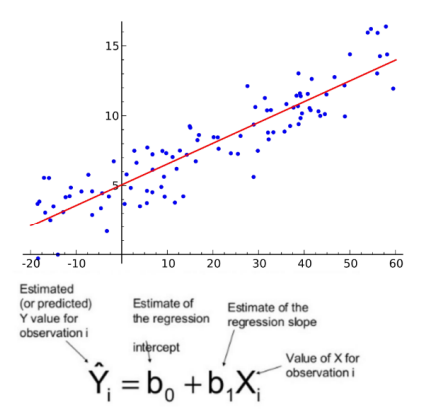
\includegraphics[scale=0.7]{reg.png}
\end{center}


Проводим гиперплоскость, наиболее хорошо разделяющую все объекты на 2 класса

\begin{center}
    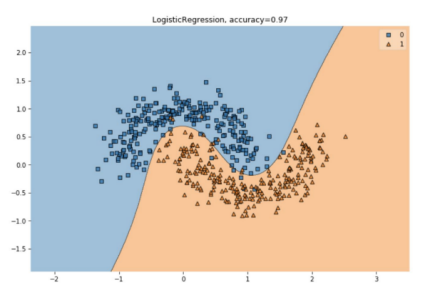
\includegraphics[scale=0.7]{images/classify.png}
\end{center}



\section{How to measure quality in classification: accuracy, balanced accuracy, precision, recall, f1-score, ROC-AUC, multiclass extensions}
\textbf{Метрики качества в задачах классификации}
\\
\textbf{1. Accuracy}\\
Accuracy - доля правильных ответов при классификации.
$$accuracy =\frac{true \ answers}{all \  answers} = \frac{T}{T + F}$$
\\
Accuracy бесполезна в задачах с неравными классами
\\

\textbf{Пример}
 Допустим, мы хотим оценить работу спам-фильтра почты. У нас есть 100 не-спам писем, 90 из которых наш
классификатор определил верно (True Negative = 90, False Positive = 10), и 10 спам-писем, 5 из которых классификатор
также определил верно (True Positive = 5, False Negative = 5). Тогда: accuracy =
$\frac{5+90}{5+90+10+5}$ = 86.4.
Однако если мы просто будем предсказывать все письма как не-спам, то получим более высокую accuracy: $\frac{0+100}{0+100+0+10}$ =
90.9
\\
\\
\textbf{2. Balanced accuracy} \\
Также есть ещё balanced accuracy. Когда мы знаем, что нам важны все классы, но мы знаем, что у одного
класса маленький размер. В таком случае мы можем сбалансировать и посчитать accuracy для каждого класса,
и уже полученные accuracy (их будет столько сколько классов) усреднить между собой. Но в реальной жизни
такая метрика оказывается довольно бесполезной, так как в такой агрегации нужно смотреть ещё на дисперсию, потому что повышая среднее, можно повысить еще и дисперсию (то есть у кого-то густо, у кого-то пусто).
Проблему дисбаланса классов такая метрика решает не очень хорошо.
$$balanced \ accuracy = \frac{1}{\#classes} \sum\limits_{\#classes} accuracy_i$$
\\
\\
 \textbf{4. Precision}\\
Precision - точность (классификация на 2 класса).(количество сбитых самолётов / общее количество выстрелов).
Количество правильных положительных ответов / общее количество положительных ответов.
\\
\begin{itemize}
    \item TP - истинно положительные
    \item FP - ложно положительные
    \item FN - ложно отрицательные
    \item TN - истинно отрицательные
\end{itemize}
\begin{center}
    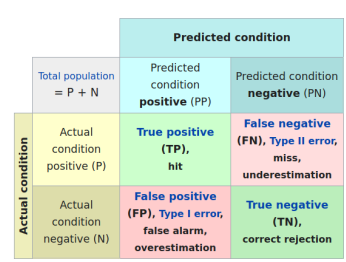
\includegraphics[]{2_1.PNG}
\end{center}
$$precision = \frac{TP}{TP+FP}$$
\\
\\
  \textbf{5. Recall}
\\
Recall - полнота. (количество сбитых самолётов / общее количество самолётов). Количество правильных положительных ответов / каким должно было быть количество положительных ответов.
$$recall =\frac{TP}{TP + FN}$$

Precision и recall не зависят, в отличие от accuracy, от соотношения классов и потому применимы в условиях несбалансированных выборок
\\
\\
\textbf{6. F-score}
\\
У нас есть две принципиально разных метрики - precision и recall, мы хотим минимизировать и ошибку 1 рода,
и ошибку 2 рода. Поэтому нам придется рассматривать то одну, то другую, как-то по очереди минимизировать,
это неудобно рассматривать две метрики одновременно. Соединим в себе две метрики, и будем брать минимум из них. Чуть-чуть подняв recall, мы чуть-чуть поднимаем precision. Такая метрика не дифференцируема
\begin{center}
    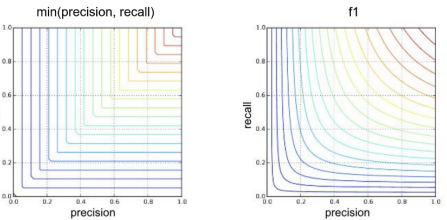
\includegraphics[]{2_2.PNG}
\end{center}
поэтому нам нужна более гладкая функция. Так появилась F1-score - гармоническое среднее между precision
и recall. Линии уровня имеют разный цвет, цветом отмечены различные значения f1-score. В правом верхнем
углу - идеальная ситуация.
$$F1 = 2\frac{1}{\frac{1}{precision}  + \frac{1}{recall}} = \frac{2 \cdot precision \cdot recall}{precision + recall}$$
\\
Как сделать так, чтобы важность precision и recall можно было пофиксить?
Например, вы решаете задачу машинного обучения в медицине, и вы хотите выделить людей, которые имеют
страшную болезнь. Вам выгоднее с точки зрения человеческих жизней, пресдказать лучше ложно человеку, что
он болен, чем пропустить человека и сказать больному, что он здоров. Таким образом recall для нас становится
важнее в этом примере.
Чтобы использовать F-score надо сдвинуть баланс, чтобы этот баланс соблюсти, у нас появляется параметр $\beta$.
$$F_{\beta} = (1 + \beta^2)\frac{  precision \cdot recall}{\beta^2 precision + recall}$$
\\
Член $1 + \beta^2$ нам нужен для нормировки, чтобы метрика оставалась между 0 и 1. Чтобы у нас был важнее
recall мы делаем $\beta < 1$ в знаменателе. В числителе обе метрики равнозначны.
\\
\\
\textbf{7.  ROC-AUC}\\
Если алгоритм бинарной классификации выдает не 0 и 1, а «вероятность 1», то чтобы дать конкретные ответы,
нужно выбрать порог. Чтобы оценивать алгоритм независимо от этого порога есть roc-auc. В нем перебирается этот
порог, и для каждого порога на графике откладываются точки (FPR, TPR). Получится ROC-кривая. Теперь чтобы
получить число, считается площадь под графиком AUC (area under ROC curve).
ROC-кривая - зависимость TPR (True Positive Rate) от FPR (False Positive Rate).
$$TPR = \frac{TP}{TP + FN}$$
$$FPR = \frac{FP}{FP + TN}$$
\\

\begin{center}
    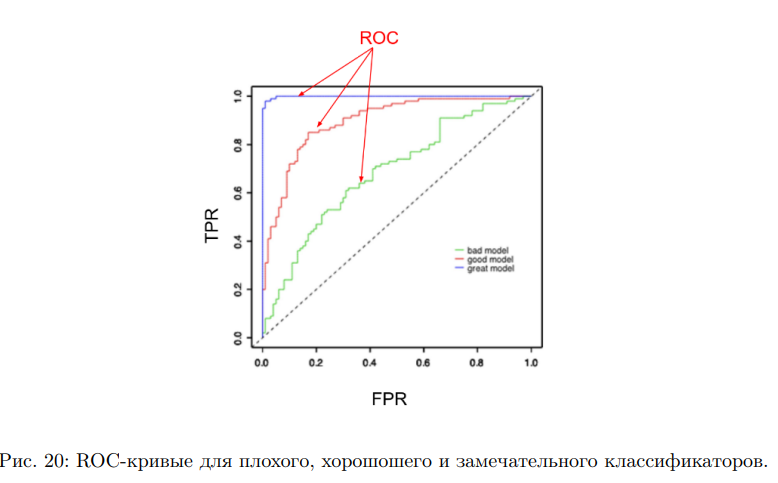
\includegraphics[]{2_4.PNG}
\end{center}
\\
\\
Главные свойства ROC кривой:
\begin{enumerate}
    
\item Baseline ялвяется случайным предсказанием, и лежит на линии y = x (диагонали на графике).
\item  Нормальный классификатор, который предсказывает что-то разумное, будет выше диагонали. Понятно,
что любой классификатор хороший, лучше чем случайное угадывание.
\item  Если предсказание лежит ниже baseline, то надо просто поменять знак, и тогда получится хороший
классификатор, кривая отразится относительно y = x.

\item Если график ROC одного классификатора строго выше (во всех точках) графика другого классификатора, то тот классификатор, который выше - лучше.
\item
Количество отсечек (ступенек) на кривой равно количеству объектов (не больше его). Если сетка установлена чаще, чем количество объектов, вы не получите ничего интересного
\end{enumerate}
\\
\textbf{Площадь под кривой ROC.} \\
Всё согласуется с тем, что мы постулировали, что чем выше кривая ROC, тем
лучше классификатор - площадь под кривой тоже будет больше. Тогда сложную кривую мы сведем к 1 числу.
По этому числу уже можно ранжировать модели между собой.
\begin{enumerate}
    \item Лежит в промежутке [0,1], но эффективно в [0.5,1], т.к. baseline имеет ROC-AUC = 0.5.
    \item Из того, что кривая лежит в каждой точке выше другой кривой, следует, что ROC-AUC у неё выше.
\end{enumerate}
Но наоборот не следует! Бывают случаи, когда один классификатор лучше в одной области, а другой в
другой области, а ROC-AUC у них равны.
\\
\\
\textbf{8.} \textbf{Мультиклассовые метрики}\\
Все предыдущие метрики были введены для бинарной классификации, чтобы перейти к метрикам мультиклассовой классификации, требуется взять среднее в каком-то смысле от метрик для всех бинарных классификаторов в мультиклассовой задаче. Буква S - сэмпл, то есть это вся выборка, а буква L - классы. В таблице показаны варианты мультиклассовых метрик из библиотеки sklearn.
\begin{center}
    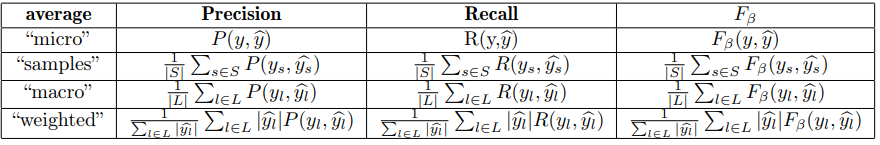
\includegraphics[]{2_5.PNG}
\end{center}




\section{How to measure quality in regression: MSE, MAE, R2.}
\ \\\textbf{1. MSE}
\\MSE - mean squared error. Среднеквадратичное отклонение прогноза от исходного значения. Сильнее штрафует за
бОльшие по модулю отклонения.
$$MSE =\frac{1}{n}\sum\limits_{i=1}^{n}(Y_i -\hat{Y_i})^2$$
где $\hat{Y}$ - предсказанный результат, Y - реальный.
\\
\\
\textbf{2. MAE}
\\
MAE - mean absolute error. Отклонение прогноза от исходного значение, усреднённое по всем наблюдениям.
$$MAE =\frac{1}{n}\sum\limits_{i=1}^{n}|Y_i -\hat{Y_i}|$$
Среднеквадратичный функционал сильнее штрафует за большие отклонения по сравнению со среднеабсолютным, и
поэтому более чувствителен к выбросам.
Среднеквадратичная ошибка подходит для сравнения двух моделей или для контроля качества во время обучения, но
не позволяет сделать выводов о том, насколько хорошо данная модель решает задачу. Например, MSE = 10 является очень
плохим показателем, если целевая переменная принимает значения от 0 до 1, и очень хорошим, если целевая переменная
лежит интервале (10000, 100000).
\\
\\
\textbf{3. $R^2$} 
$$R^2 = 1 -
\frac{\sum\limits_{
i=1}^{n}(Y_i - \hat{Y_i})^2}{\sum\limits_{
i=1}^{n}(Y_i - \overline{Y})^2}$$

Член вычитаемый из 1 можно интерпретировать как оценённую дисперсию, отнесённую к реальной дисперсии. Ещё можно сказать, что мы модель сравниваем с моделью, которая предсказывает просто константу. Смотрим насколько далеко ушла наша модель от тупого предсказания среднего.
Может иметь отрицательные значения, так как числитель может неограниченно расти.
\begin{unnecessary}
\ \\
\textbf{MAPE}\\
$$MAPE =\frac{1}{n}\sum\limits_{
i=1}^{n}|\frac{Y_i - \hat{Y_i}}{Y_i}|$$
\\
\textbf{SMAPE}
\\
 Когда есть большие выбросы в MAPE, следует
использовать отнормированную и на прогнозируемое значение метрику.
$$SMAPE =\frac{1}{n}\sum\limits_{
i=1}^{n}\frac{2|Y_i - \hat{Y_i}|}{|Y_i| + |\hat{Y_i}|}$$
\end{unnecessary}


\section{ Maximum likelihood estimation, how is it related to regression and classification}
Функция правдоподобия это ни что иное как условная вероятность выборки, при условии что
параметрические семейство, которое описывает эту выборку обладает ровно таким параметром.
$$L(\theta | X, Y ) = P(X, Y |\theta)$$
От правдоподобия мы хотим только одну вещь - максимизировать. Хотим наиболее правдоподобные параметры
при условии нашей выборки.
$$L(\theta | X, Y ) \rightarrow \underset{\theta}{\max}$$
Так как матрица признаков имеет незаивисимые объекты i.i.d, мы можем расписать условную вероятность
как произведение условной вероятности по каждому объекту.
$$L(\theta|X, Y ) = P(X, Y |\theta) = \prod\limits_i P(x_i, y_i |\theta)$$
Argmax функции совпадает с argmax любого монотонного преобразования над функцией. Тут можно использовать логарифм, который из произведения делает сумму, логарифм - монотонное преобразование, поэтому
мы можем заменить произведение на сумму логарифмов условной вероятности и его уже максимизировать:
$$log L(\theta|X, Y ) = P(X, Y |\theta) = \sum\limits_i log P(x
_i, y_i |\theta)  \rightarrow \underset{\theta}{\max}$$
\\
\begin{note}
ФУНКЦИЯ ПРАВДОПОДОБИЯ - ЭТО НЕ РАСПРЕДЕЛЕНИЕ НАД ПАРАМЕТРАМИ $\theta$

\end{note}

\begin{note}
\
\\

Большинство моделей работает по принципу максимального правдоподобия, линейная регрессия и классфикация работают именно по нему.

В задаче линейной регресси мы ходим минимизировать MSE для получения оптимального вектора весов. Задача минимизации MSE эквивалентна методу максимального правдоподобия при определенных условиях по теореме Гаусса-Маркова.
\\
В задаче классификации мы напрямую используем MLE для выбора параметров
\end{note}



\section{Naive bayesian classifier, how does it work}
Наивное предположение: фичи независимы. 

Вспомним теорему Байеса, которая дает нам формулу условной вероятности:

$P(A|B) = \frac{P(B|A)P(A)}{P(B)}$

Ставится задача $K$-классовой классификации (то есть каждый элемент по какому-то признаку может быть одного из $k$ возможных классов). $$x_i \in \R^p, y_i \in \{C_1, \dots, C_k\}$$

Давайте прикинем условную вероятность метки класса при условии того, что объект описывается какими-то фичами.

$$P(y_i = C_k|x_i) = \frac{P(x_i|y_i = C_k)P(y_i = C_k)}{P(x_i)}$$

То есть мы оцениваем, какова вероятность того, что метка класса это $C_k$ при условии, что мы наблюдаем $x_i$.

Уже имея данную формулу мы можем оценивать вероятность лейблов. $P(y_i = C_k)$ оценим как частоту (встречаемости) каждого класса в нашей выборке (просто руками посчитаем, насколько вероятно попадание в тот или иной класс). Но нам надо оценить $P(x_i|y_i = C_k)$. Это сделать непонятно, как, потому что $x_i$ -- это вектор. Здесь и понадобится наше \textit{наивное} предположение - все признаки независимы и тогда хорошо факторизуются (мы считаем, что признаков у нас $p$).

$$P(x_i|y_i = C_k) = \prod\limits_{n = 1}^p P(x_i^n|y_i = C_k)$$

В реальной жизни признаки часто зависимы, причем они бывают зависимы довольно сложным образом, так что просто так взять и подчистить данные не удастся. Но есть хорошая новость -- признаки бывают частично независимы (например, среди них бывают независимые подмножества), так что какой-то смысл в этом есть. Теперь вектор $x_i$ представляется как вектор $p$ независимых случайных величин. Мы хотим найти метку класса, которая наиболее вероятна

$$C^* = \underset{k}{argmax} ~ P(y_i = C_k|x_i) = \underset{k}{argmax} ~ \frac{P(x_i|y_i = C_k)P(y_i = C_k)}{P(x_i)}$$ Это и будет нашим предсказанием.\\

Теперь заметим, что знаменатель не зависит от $k$, поэтому на нахождение максимума он не влияет. То есть если его убрать, у нас, конечно, выражение перестанет быть вероятностью, но метка класса, при котором достигается этот самый максимум, не изменится. Поэтому на него можно забить, и даже сэкономить на этом какое-то время (хотя и не очень большое).

Правда, на самом деле, мы в любом случае его и так практически посчитаем по пути, так как $P(x_i) = \sum_kP(x_i|y_i=C_k)$.\\

Для того, чтобы посчитать $P(x_i^l|y_i = C_k)$, требуется ввести какое-то распределение на наши признаки. Строго понять это вряд ли получится, так что или нам это было известно, или мы должны просто предположить, из какого распределения они пришли. Тут есть 2 пути: 1 - если они тоже все категориальные, можем просто посчитать частоту каждого из них, 2 - если они какие-то числовые, то тут чуть сложнее, нам придется ввести какое-то априорное распределение на $x$. Самый простой случай, когда $x$ пришел из нормального распределения. В этом случае мы считаем дисперсию и среднее по выборке, предполагая что распределение нормальное, и тогда можем оценить вероятность.

Такой классификатор будет хорошо работать на классификации текстов (например, определять, грубый ли комментарий в соц.сети).

\section{K-nearest neighbours classifier, how does it work}
\subsection*{Интуиция и идея kNN}

\begin{example}
Рассмотрим картинку. Путь у нас все объекты двух типов -- синий квадрат или красный треугольник. И вот нам поступил объект, который на картинке отмечен зеленым кружочком. Мы про него хотим понять, кто он на самом деле (к какому из двух классов относится). Это несложно делается с помощью метода ближайших соседей.
\end{example}

\begin{center}
    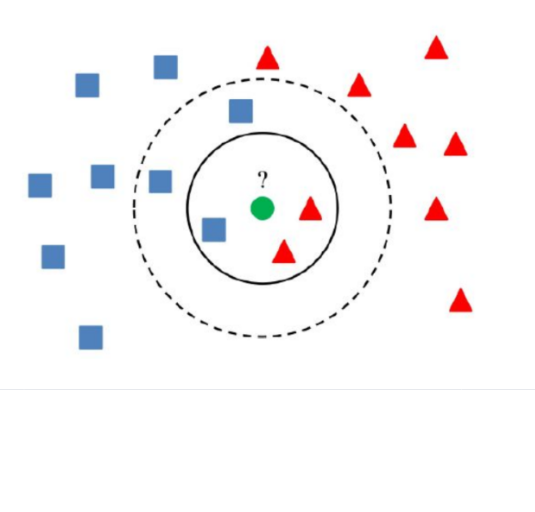
\includegraphics[scale=0.7]{images/6_1.png}
\end{center}

Собственно, плюс метода ближайших соседей как раз в том, что он абсолютно интуитивный. Идея такая: <<чем ближе я к другим объектам в признаковом пространстве, тем больше я на них похож>>. 
Мы можем использовать расстояние между объектами в пространстве признаков как некоторую меру похожести.

Допустим на картинке мы будем считать расстояние по $L2$-норме, то есть использовать Евклидово расстояние, к которому мы привыкли. В этой и других задачах в прицнипе можно ввести любую другую метрику и по ней посчитать расстояние.

Если у нас просто есть выборка, и она желательно задана в каком-то линейном метрическом пространстве, то, как правило, там мало категориальных фичей, этим можно воспользоваться и применить собсвенно описанную выше идею. Вот тут появляется выбор гиперпараметра модели: тут это параметр $k$ -- сколько ближайших соседей мы выбираем для того, чтобы решить, к какому классу относится объект. Если мы возьмем одного соседа, он может оказаться выбросом из выборки и дать нам неверный результат. Но если мы возьмем информацию о нескольких соседях, мы будем более уверены в предсказании класса объекта. 

\begin{example}[Пример из жизни, поясняющий интуицию:]
Так, например, если вокруг вас вечером много физтехов, то вы, скорее всего, студент физтеха и находитесь в общежитии. 
\end{example}

\subsection*{Алгоритм kNN}

В итоге получаем такой алгоритм:

\begin{enumerate}
    \item Берем датасет и запоминаем координаты объектов в пространстве признаков.
    \item Берем новое наблюдение и считаем все расстояния до каждого объекта в датасете.
    \item Выберем $k$ объектов с минимальным расстоянием до вашего нового наблюдения.
    \item Выбираем класс, который доминирует среди этих $k$ соседей. Он-то и будет нашим предсказанием для рассматриваемого объекта.
\end{enumerate}

Есть минусы в таком подходе:

\begin{enumerate}
    \item При разных значениях гиперпараметра числа соседей может получаться различный результат. Можем проверять качество работы алгоритма при фиксированном параметре, но не можем сходу оптимизировать его (оптимизируется только перебором, к сожалению).
    \item В настоящее время при больших выборках занимает большое вычислительное время из-за подсчета большого количества расстояний (а в пространствах с большой размерностью расстояния считаются между длинными векторами, что тоже долго, все ведь помним плюсы с длинной арифметикой :) ).
\end{enumerate}


\subsection*{Взвешенный kNN}

Теперь подумаем, как еще мы можем предсказывать класс на основе информации о $k$ ближайших сосседях. Сейчас мы выбираем самый часто встречающийся класс, но, может быть, можно делать лучше? Есть такой выход.

Он называется взвешенным $kNN$. В этой вариации мы  присваиваем вес лейблу каждого соседа в зависимости от расстояния от нашего объекта до соседа. То есть чем дальше сосед, тем меньший вклад в ответ он вносит.

\subsection*{Как с помощью $kNN$ решить задачу регрессии?}

Практически ничего не меняется, только таргетами станет континуальная величина, то есть числа.
Что надо сделать с матрицей признаков перед тем как использовать на ней $kNN$?

Ее обязательно надо отнормировать. 

\begin{example} Если в одной матрице есть признак в сантиметрах и признак в метрах, то это странно. Или в бухгалтерии зарплата представлена в матрице в рублях и в копейках как два разных признака, то 
по-хорошему их надо объединить в один признак или привести в одну шкалу, то есть чтобы были рубли и доли рублей. 
\end{example}

Если мы ничего не знаем о природе нашей выборки, то самое лучшее, что мы можем с ней сделать, это отнормировать ее в промежуток $[0;1]$, то есть вычесть минимум и поделить на максимум.

\section{Linear regression. Problem statement for the MSE loss function case. Analytical solution. Gauss-Markov theorem. Gradient approach in linear regression.}
\textbf{Постановка задачи}

Пусть задан датасет \( \mathcal{L} = \{x_i, y_i\}_{i = 1}^N\),
где \(x_i \in \R^n, y_i \in \R\).
Наша модель линейная, то есть предсказание выглядит следующим образом:

\[
\widehat{y} = w_0 + \sum_{k = 1}^p x_k \cdot w_k = x^T w
\]

Чтобы отдельно не записывать свободный член, добавим в $x$ признак, тождественно равный единице. Тогда соответствующий коэффициент в $w$ будет отвечать за свободный член:

\[
\begin{pmatrix}
1 & x_1 & \ldots & x_p
\end{pmatrix}
\begin{pmatrix}
w_0 \\
w_1 \\
\ldots \\
w_p
\end{pmatrix}
= w_0 + \sum_{k = 1}^p x_k \cdot w_k
\]

Задача оптимизации, которую мы решаем -- это минимизация какого-то функционала. Например, среднеквадратичной ошибки (такой подход называется методом наименьших квадратов):

\[
\widehat{w} = \arg \min_w \|Y - \widehat{Y}\|_2^2 = 
\arg \min_w \|Y - Xw\|_2^2
\]

В случае минимизации среднеквадратичной ошибки существует аналитическое решение:

\begin{multline*}
\|Y - Xw\|_2^2 = \langle Y - Xw, Y - Xw \rangle = 
Y^T Y - (Xw)^T Y - Y^T (Xw) + (Xw)^T Xw = \\
= Y^T Y - w^T X^T Y - Y^T X w + w^T X^T X w
\end{multline*}

\[
\nabla_w \|Y - Xw\|_2^2 = 0 - X^T Y - X^T Y + 
\left( X^T X + X^T X \right) w
\]

Приравнивая \(\nabla_w \|Y - Xw\|_2^2\) к нулю, получаем:

\[
\widehat{w} = (X^T X)^{-1} X^T Y
\]

\begin{note}
Аналитическое решение существует только для 2-нормы. Для остальных норм решение ищется только градиентными методами.
\end{note}

\begin{theorem}[Гаусса-Маркова]
Пусть целевые значения выражаются в следующем виде:

\(Y = Xw + \varepsilon\), где 
\(\varepsilon = (\varepsilon_1, \ldots, \varepsilon_N)\) -- случайный вектор, при этом:

\begin{enumerate}
    \item \(\mathbb{E} \varepsilon_i = 0\ \forall i\)
    \item \(\mathbb{D} \varepsilon_i = \sigma^2 < \infty\ \forall i\)
    \item \(\text{cov}(\varepsilon_i, \varepsilon_j) = 0\ \forall i \neq j\)
\end{enumerate}

Тогда решение задачи наименьших квадратов 
$\widehat{w} = (X^T X)^{-1} X^T Y$ является оптимальным среди несмещённых.

Другими словами, $\widehat{w}$ является несмещённой (\(\mathbb{E} \widehat{w} = w\)) и оптимальной (то есть имеет наименьшую дисперсию среди всех несмещённых).

\textbf{Основные функции потерь в регрессии}

\[
\text{MSE}(y, \widehat{y}) = 
\frac{1}{N} \|y - \widehat{y}\|_2^2 = 
\frac{1}{N} \sum_i (y_i - \widehat{y_i})^2
\]

\begin{itemize}
    \item Применима теорема Гаусса-Маркова
    \item Дифференцируема
    \item Чувствительна к шуму
\end{itemize}

\[
\text{MAE}(y, \widehat{y}) = 
\frac{1}{N} \|y - \widehat{y}\|_1 = 
\frac{1}{N} \sum_i |y_i - \widehat{y_i}|
\]

\begin{itemize}
    \item Не дифференцируема (можно доопределить производную в нуле нулём)
    \item Более устойчива к шуму
\end{itemize}

\end{theorem}


\section{Regularization in linear models: L1 и L2, their properties. Probabilistic interpretation.}
Напомним, что аналитическое решение для метода наименьших квадратов выглядит следующим образом:

\[
\widehat{w} = (X^T X)^{-1} X^T Y
\]

Видно, что нам приходится искать матрицу, обратную к $X^T X$. Однако, что делать, если эта матрица вырождена (или близка к вырожденной)? 

Сначала подумаем, что означает вырожденность матрицы $X^T X$. Это означает, что в этой матрице (а значит, и в матрице $X$) есть линейно зависимые столбцы (признаки). В таком случае столбец весов не может быть определён однозначно, так как будет фиксирована только сумма весов этих параметров, а сами параметры могут определяться континуальным количеством способов.

Если же матрица $X^T X$ близка к вырожденной, то решение получается \textit{нестабильным} (то есть при добавлении небольшого шума в данные вектор весов меняется сильно).

Чтобы решить эту проблему, нам хочется ограничить свободу выбора этих коэффициентов, наложить дополнительное условие, чтобы решение стало единственным. Давайте потребуем, чтобы норма вектора весов была наименьшей из возможных. Тогда задача оптимизации запишется следующим образом:

\[
\widehat{w} = \underset{w}{\argmin}
\left( \|Y - Xw\|_2^2 + \lambda \|w\|_2^2 \right)
\]

Коэффициент $\lambda$ -- это гиперпараметр, который отвечает за то, насколько важно для нас, чтобы норма вектора весов была маленькая.

\textbf{Важное замечание.}
В слагаемом \(\lambda \|w\|_2^2\) мы записываем $w$ без свободного члена ($w_0$), так как иначе наша модель будет стараться уменьшать в том числе и $w_0$, то есть пытаться провести гиперплоскость через ноль. В общем случае это не следует не из каких предположений, поэтому накладывать ограничение на $w_0$ нельзя.

Аналитическое решение такой задачи будет выглядеть следующим образом:

\[
\widehat{w} = \left( X^T X + \lambda I \right)^{-1} X^T Y
\]

Видно, что теперь обратная матрица существует всегда (так как  к $X^T X$ мы добавляем единичную матрицу).

Подход, при котором мы накладываем дополнительные ограничение, называется \textit{регуляризацией}. При этом не обязательно накладывается ограничение на норму вектора весов (см. другие примеры в билете \ref{27}).

Можно применять не только $L2$ регуляризацию, но и $L1$.

\textbf{L2}
\begin{itemize}
    \item имеет аналитическое решение
    \item дифференцируема
\end{itemize}

\textbf{L1}
\begin{itemize}
    \item не дифференцируема
    \item "отбирает" признаки
\end{itemize}

\section{Logistic regression. Equivalence of MLE approach and logistic loss minimization.}
\textbf{Постановка задачи}

$X \in \R^{n \times p}, Y \in C^n$, где $C$ -- это множество меток классов (конечное). Если метки не упорядочены, то это называется \textit{задачей классификации}.

Пока что будет заниматься бинарной классификацией и для удобства будем считать, что \(C = \{-1, 1\}\). Обозначим за $c(X)$ функцию, которая возвращает $\widehat{Y}$, то есть предсказание классов нашей модели.

Допустим у нас есть матрица признаков и вектор весов, как из этого всего, что уже было в линейной регрессии,
составить линейную классификацию?
Надо делить на классы предсказанный ответ, обрубая по какой-то границе, если у нас два класса.

\[
c(x) = 
\begin{cases}
1, f(x) \geqslant 0 \\
-1, f(x) < 0
\end{cases}
\]

Пусть вектор $w$ является нормалью к гиперплоскости в $p$-мерном пространстве фичей (гиперплоскость задаётся уравнением $x^T w = 0$), с одной стороны гиперплоскости будут одного класса объекты, с другой --- другого класса объекта. Тогда $c(x)$ можно переписать в следующем виде:

\[
c(x) = \sgn(f(x)) = \sgn(x^T w)
\]

Введём понятие margin (отступ):

\[
M_i = y_i f(x_i) = y_i x_i^T w
\]

Это некоторый аналог ориентированного расстояния, причём если $M_i \leqslant 0$, значит объект классифицирован неправильно. Тогда логично предложить следующую функцию потерь:

\[
\text{Loss} = \sum_{\text{by objects}} [M_i \leqslant 0]
\]

Но у такой loss function будут проблемы, так как это не гладкая функция. Это главная причина почему мы
не будем использовать такой loss, по крайней мере в наших текущих задачах. Есть ещё один менее очевидный
минус: такая метрика ничего нам не говорит об уверенности классификатора. Представьте объекты как точки
в пространстве признаков, есть гиперплоскость классификатора, и было бы разумно полагать, что объекты
на границе, где перемешиваются два класса, будут с меньшей уверенностью разделены классификатором, чем
лежащие далеко "в толще"класса, которые с большей точностью принадлежат своему классу.

Что можно сделать с имеющейся функцией потерь --- приблизить её к гладкой функции. Предлагается использовать логистическую регрессию.

\[
p_+ = P(y = 1|x) \in [0, 1]
\]

Регрессионная модель живет в пространстве $\R$, а вероятность живёт исключительно в промежутке [0,1]. Как с этим быть?
Применить функцию, которая переводит R в промежуток [0,1] и таким образом моделлирует вероятность.
Используем некий трюк и составим величину, которая уже будет куда ближе к R:
$\frac{p_+}{1 - p_+} \in [0, +\infty)$

Осталось отразить промежуток $[0, +\infty]$ в $\R$, с чем хорошо справляется функция логарифма:
$\log \frac{p_+}{1 - p_+} \in \R$
Таким образом мы объединили мир классификации и мир регрессии. Теперь запишем предсказание через
вектор признаков и вектор весов, а также выразим вероятность объекта иметь класс 1:
\[
\frac{p_+}{1 - p_+} = \exp(x^T w)
\]
\[
p_+ = \frac{1}{1 + \exp(-x^T w)} = \sigma(x^T w)
\]
Получилось, что вероятность объекта иметь 1 класс равна сигмоиде от привычного выражения для линейной
регрессии.

\section{Multiclass classification. One-vs-one, one-vs-all, their properties.}
Что делать, если мы хотим классифицировать объекты не на два класса, а на большее количество? Есть два разных подхода

\textbf{One vs Rest}

Исходя из названия понятен смысл: мы берём один класс, все остальные объекты помечаем другим классом.
Далее на этом тренируем классификатор, потом берём следующий класс, кроме этого второго класса, помечаем
остальные объекты противоположным классом. И так тренируем столько классификаторов, сколько у нас есть
классов.

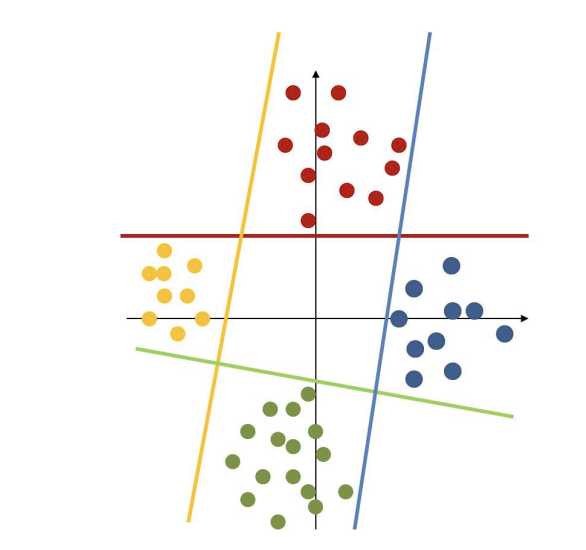
\includegraphics{images/10_1.png}

Довольно очевидно, что тот, у кого наибольшая вероятность в таком процессе, предсказывается следующим
образом: берётся точка в пространстве, мерим вероятности относительно каждого из построенных классификаторов и смотрим у кого больше вероятность, к тому классу мы и относим. Как должны быть расположены
классы в пространстве признаков, чтобы поломать такой классификатор?
Центры каждого класса должны быть расположены на одной прямой, такая ситуация поломает подобную
классификацию.
Понятно, что крайние два класса будут хорошо разделяться, а средний не будет отделяться вообще никак,
потому что нельзя линейным классификатором (одной гиперплоскостью) отделиться от двух других классов
справа и слева.

Есть ещё одна проблема, которая менее заметна на первый взгляд: серые зоны. На рисунке серую зону
можно увидеть в центре. Если в ту область попадают объекты из обучающей выборки, непонятно к какому
классу их отнести, у нас нет таких данных. Равно как и в остальных серых зонах по бокам, тоже непонятно
что будет происходить. В достаточно простом случае мы можем это предсказать - финальное решение поделит
серые зоны между каждыми двумя классификаторами пополам, а в центре на столько частей сколько классов
всего. Несовпадение границ проведенных и границ финальных связано с тем, что мы принимаем решение
коллективно.

\textbf{One vs One}

В такой стратегии мы будем сравнивать один класс с каким-нибудь другим классом из имеющихся, применяя
опять линейный классификатор. 

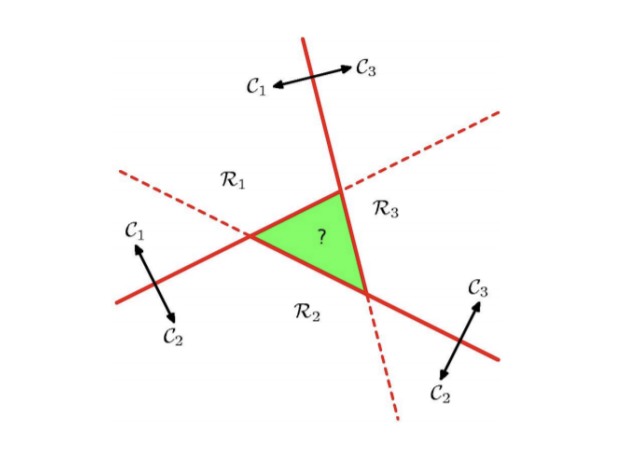
\includegraphics{images/10_2.png}

Буквами $R_i$ на картинке обозначены кластера тех объектов, которые мы будем классифицировать. А сплошные линии, переходящие в пунктирные это классификаторы. Класс $c_2$
отделяется классификатором от класса $c_1$, не смотря совершенно на класс 3, и тд.

\textbf{Сравнение}

В одном случае мы тренируем только $k$ классификаторов, но тренируем их на полном датасете каждый --- это отражается на времени обучения всего классификатора. Во втором случае
мы тренируем квадратичное число классификаторов, но с другой стороны у нас есть плюс в том, что если
классы равномерно распределены, то каждый раз мы будем только два кластера из всех рассчитывать (то
есть меньше чем весь датасет). Но в стратегии one vs one есть проблема в том, что слишком мало сэмплов. То
есть существуют классы, которых меньше в выборке, и с ними может возникнуть проблема.
Надо заметить, что в таком процессе one vs one мы убираем строки из матрицы признаков, а не столбцы, то
есть количество признаков сохраняется, а именно количество объектов при обучении уменьшается.

\section{Support vector machine. Optimization problem for SVM. Kernel trick. Kernel properties.}
\textbf{Мотивация:}\\

Ранее мы рассматривали логистическую регрессию и log loss в виде логарифма от сигмоиды. Но данную задачу приближения loss function гладкой функцией можно решать и другими способами, один из них - SVM.\\

Давайте начнём с простого случая, когда у нас есть линейно разделимая выборка (хотя на практике такое вряд ли произойдет). Подумаем, как выбрать оптимальную гиперплоскость, которая разделяет два класса. Вопрос в том, что таких гиперплоскостей может быть очень много (например, какую-нибудь подходящую гиперплоскость можно чуть-чуть или даже не чуть-чуть пошевелить). \\

Получается, что много моделей представляют решение одной и той же задачи классификатора, и одно и то же значение эмпирического риска. В итоге у нас решение не единственно, а это плохо, потому что непонятно тогда, какое выбирать. \\

\begin{center}
    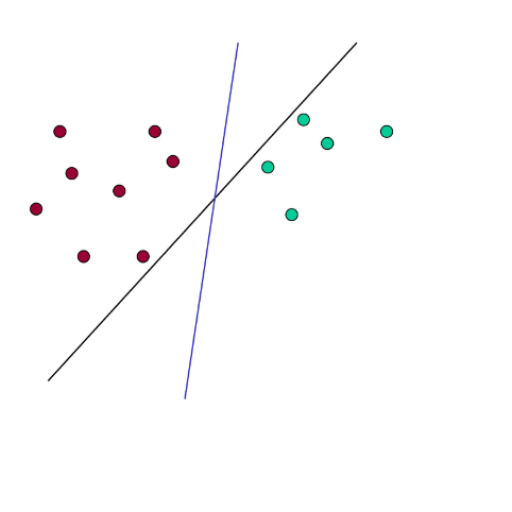
\includegraphics[scale=0.7]{images/11_1.png}
\end{center}

\textbf{Идея:}\\

Поэтому давайте поймем, какая модель (гиперплоскость) линейной классификации лучше? Полезно не только строить гиперплоскости, но и максимизировать ширину зазора между классами, которую эта гиперплоскость определяет (собственно, интуитивно кажется, что так разделение будет качественнее всего).

$$\exists w, w_0 : M_i(w, w_0) = y_i(\langle w, x_i \rangle - w_0) > 0 \forall i \in \{1, \dots, l\}$$

Формула выше представлена для ситуации, когда $bias$ не включен в вектор весов, и в вектор признаков не включена в начале $1$. Поэтому мы вычитаем ещё смещение $w_0$.

Если умножить гиперплоскость на константу, наклон не поменяется, поэтому мы можем произвести нормировку (никогда не было, и вот опять) $margin$ в $1$ с помощью изменения параметров модели $w$.

Раеммотрим следующую картинку: 

\begin{center}
    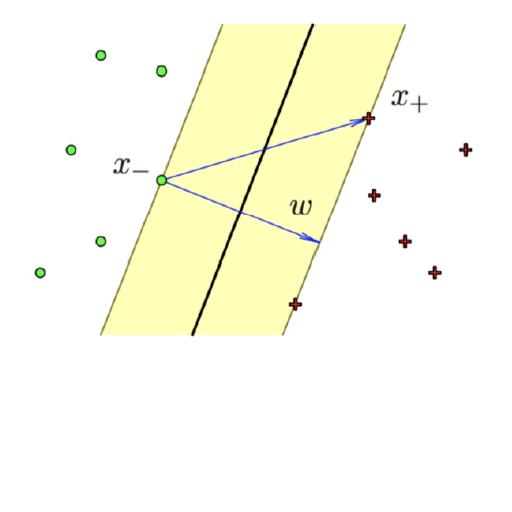
\includegraphics[scale=0.7]{images/11_2.png}
\end{center}

Отступ на ней это значение вектора $w_0$. Будем считать, что для самого левого красного плюсика (если смотреть на расстояние до гиперплоскости) у нас верно $\langle w, x_+ \rangle - w_0 = 1$. Тогда все точки правее будут иметь $\langle w, x \rangle - w_0 \geqslant 1$, а все точки левее самого правого зеленого кружочка будут
иметь $\langle w, x \rangle - w_0 \leqslant -1$. 

Мы хотим максимизировать ширину полосы между классами. Тогда давайте максимизировать, вспоминая линейную алгебру и то, как оценить расстояние от точки до прямой. Будем максимизировать расстояние между крайней левой точкой <<положительного>> класса, и крайней правой точкой <<отрицательного>> класса.

$$\frac{\langle x_+ - x_-, w \rangle}{\|w\|} \geqslant \frac{2}{\|w\|} \to \max$$

Широкая полоса между классами хороша тем, что даже имея девиации, классификатор всё ещё будет хорошо предсказывать разделение по классам. То есть если у нас появится в выборке несколько новых объектов, наш классификатор не будет резко менять свое решение, как могло произойти ранее. Потому что теперь мы не просто ищем гиперплоскость, но и максимизируем ширину между классами объектов.
Как мы уже сказали ранее, модуль отступа должен быть положителен для каждого класса объектов с учетом нашей нормировки, так как выборка линейно разделима по нашему предположению. Максимизируем модуль расстояния между классами, значит минимизируем квадратичный функционал нормы вектора весов:

$$ \begin{cases}
   \frac{1}{2}\|w\|^2 \to \min\limits_{w, w_0}\\
   M_i(w, w_0) \geqslant 1 & i = 1, \dots, l
 \end{cases}$$

Всё было бы здорово и задача оптимизации была бы поставлена, но мы сделали одно очень далекое от правды предположение, что наша выборка линейно разделима. На практике есть шум, сложные зависимости, которые не обязательно линейно разделяются. Или объекты одного класса могут попасть в глубину объектов другого класса (случайно попасть не в свою группу, а в другую). Как их разделять теперь, непонятно. И в этом случае у нас появляется отрицательный отступ, и все ломается.

Но есть выход. Можно просто ввести некоторый штраф за то, что объект попал к объектам другого класса.\\

\begin{center}
    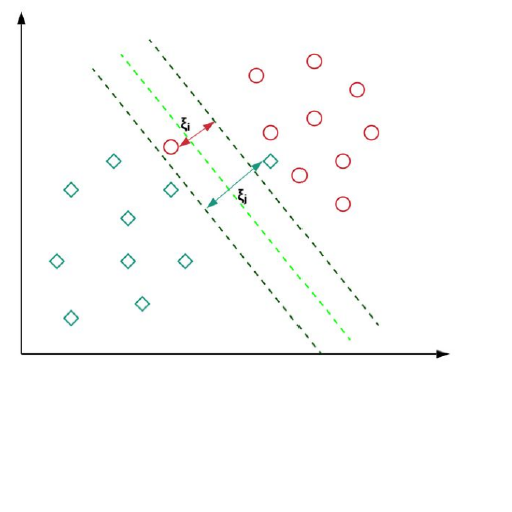
\includegraphics[scale=0.7]{images/11_3.png}
\end{center}

Новая постановка задачи будет выглядеть так (в ней $\xi_i$ как раз наш штрафной член):

$$\begin{cases}
   \frac{1}{2}\|w\|^2 + C\sum\limits_{i=1}^l \xi_i \to \min\limits_{w, w_0, \xi}\\
   M_i(w, w_0) \geqslant 1 - \xi_i & i = 1, \dots, l\\
   \xi_i \geqslant 0 & i = 1, \dots, l
 \end{cases}$$.

 Второе неравенство можем рассматривать как ограничение на $\xi_i$, если перенесем $\xi_i$ влево, а $margin$ вправо.

 Тогда, чтобы $\xi_i$ удовлетворяла обоим неравенствам (второму и третьему), нужно $\xi_i \geqslant \max(1 - M_i(w, w_0), 0)$.

 $C$ -- регуляризационная константа, которая отвечает за то, насколько сильно мы штрафуем модель.

 В итоге сумму, которую мы минимизируем, можно переписать как 

 $$C\sum\limits_{i=1}^l \max(0, 1- M_i(w, w_0)) + \frac{1}{2} \|w\|^2 \to \min\limits_{w, w_0}$$

 Правда, сейчас мы хоть и учли ограничения, но получили более сложную для решения задачу, ведь $\max(0, 1- M_i(w, w_0))$ не является гладкой функцией.\\

 Сейчас придется вспомнить методы оптимизации и теорему Каруша--Куна--Такера.

 В общем случае минимизация с заданными условиями это:

 $$\begin{cases}
   f(x) \to \min\limits_x\\
   g_i(x) \leqslant 0 & i = 1, \dots, m\\
   h_j(x) = 0 & j = 1, \dots, k
 \end{cases}$$

 Тогда у нас есть необходимые условия для локального минимума в общем случае:

 $$\begin{cases}
   \frac{\partial \mathcal{L}}{\partial w} = 0, \mathcal{L} = f(x) + \sum\limits_{i=1}^m \mu_ig_i(x) + \sum\limits_{j=1}^k \lambda_jh_j(x)\\
   g_i(x) \leqslant 0; h_j(x) = 0\\
   \mu_i(x) \geqslant 0\\
   \sum\mu_ig_i(x) = 0
 \end{cases}$$

 Можем расписать для нашего Лагранжиана:

 $$\mathcal{L}(w, w_0, \xi, \lambda, \eta) = \frac{1}{2}\|w\| - \sum\limits_{i=1}^{l} \lambda_i (M_i(w, w_0) - 1) - \sum\limits_{i=1}^{l}\xi_i (\lambda_i + \eta_i - C)$$

 Необходимые условия минимума:

 $$\begin{cases}
   \frac{\partial \mathcal{L}}{\partial w} = 0 \Rightarrow w = \sum\limits_{i=1}^l \lambda_i y_i x_i\\
   \frac{\partial \mathcal{L}}{\partial w_0} \Rightarrow \sum\limits_{i=1}^l \lambda_i y_i = 0\\
   \frac{\partial \mathcal{L}}{\partial \xi} = 0 \Rightarrow \eta_i + \lambda_i = C & i = 1, \dots, l\\
   \xi_i \geqslant 0, \lambda_i \geqslant 0, \eta_i \geqslant 0\\
   \lambda_i = 0 \vee M_i(w, w_0) = 1 - \xi_i\\
   \eta_i = 0 \vee \xi_i = 0
 \end{cases}$$

Так причём здесь метод опорных векторов (SVM)?
Делаем простое решение, в котором у нас участвуют только те объекты, которые так или иначе являются опорными объектами, то есть объектами, которые находятся около разделяющей полосы или внутри неё. Те объекты, которые лежат внутри своего класса, вообще говоря для нашего классификатора особо не играют роли, потому что та функция потерь, о которой мы говорим $\max(0, 1-M)$ реагирует только на те объекты, которые находятся внутри разделяющей полосы или в глубине чужого класса. 

Наша модель штрафуется не только в том случае, когда она неправильно проклассифицировала объект, но и за то, что они просто попали внутрь разделяющей полосы. 

\begin{center}
    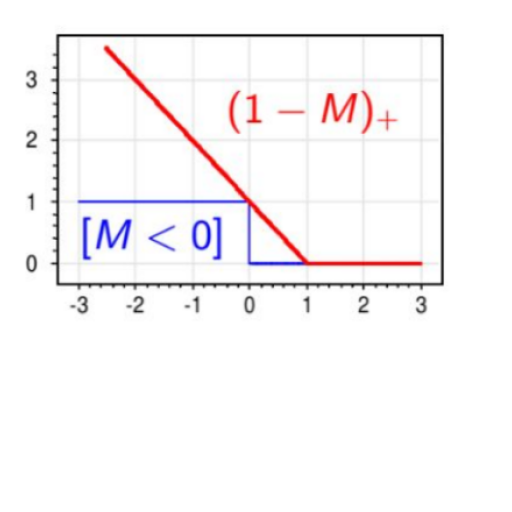
\includegraphics[scale=0.7]{images/11_4.png}
\end{center}

На картинке  наш настоящий лосс указан синей ступенькой, это тот лосс, который мы хотим минимизировать, а, значит, по рисунку видно, что тот функционал, который мы будем в итоге минимизировать, является верхней оценкой функции эмпирического риска. 

По сути, минимизируя красный функционал (Hinge loss), мы минимизируем mis loss.\\


\textbf{Теперь про регуляризацию}\\

Член функционала, состоящий из квадрата нормы вектора весов с некой константой - типичный регуляризационный член, от которого зависит ширина полосы. Напомним, что изначально мы хотели получить максимальную ширину полосы между классами. Мы пришли к привычному виду функции потерь:

$$Q(w, w_0) = \sum\limits_{i=1}^l[M_i(w, w_0) < 0] \leqslant \sum\limits_{i=1}^l \max(0, 1 - M_i(w, w_0)) + \frac{1}{2C}\|w\|^2 \to \min$$


Первое слагаемое отвечает за апроксмимацию решения, а второе - за регуляризацию. Константа $C$ в знаменателе регуляризационного члена появилась, потому что можно без нарушения общности поделить наш функционал на $C$ (заметим, что это та же $C$, что и в формулах ранее). 

Похожесть получившийся функции потерь на функцию потерь, например, в линейной регрессии, говорит нам о том, что есть общие подходы в математике построения моделей. И,  вообще говоря, добавление регуляризации привносит добавление некоего априорного знания внутрь нашей модели, в данном случае - максимизирует ширину межклассовой полосы. Так как константа стоит тут в знаменателе, то чем больше константа, тем слабее регуляризация и тем полоса уже. \\

\begin{center}
    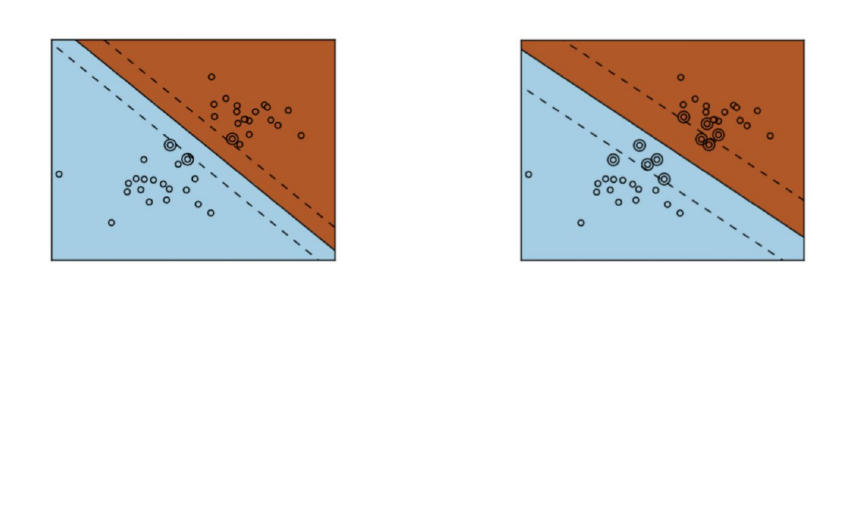
\includegraphics[scale=0.5]{images/11_5.png}
\end{center}

На этой картинке слева значение $C$ больше, справа -- меньше.

\textbf{Нелинейный SVM}\\

Внутри $margin$ лежит скалярное произведение. И, вообще говоря, мы можем использовать другое скалярное произведение, заданное для другого пространства.

Это основная идея нелинейного SVM: использовать другое преобразование для задания скалярного произведения на другом Гильбертовом пространстве. Для этого вводится функция ядра ($kernel$), которая обладает простыми свойствами. 

\begin{theorem}[теорема 1999 года Мерсера] функция может являться ядром, если она симметрична и неотрицательно определена,
$$K(x, x') : X \times X \to \R$$
$$\exists \phi : X \to H : \quad K(x, x') = \langle \phi(x), \phi(x') \rangle \text{, где } H \text{ --- шиьбертово пр-во}
$$
\end{theorem}

\begin{example}
Приведём несколько примеров ядер:

\begin{enumerate}
    \item $K(x, x') = \langle x, x' \rangle^2$
    \item $K(x, x') = \langle x, x' \rangle^d$
    \item $K(x, x') = (\langle x, x' \rangle + 1)^d$
    \item $K(x, x') = \exp((-\gamma\|x - x'\|^2)$ -- RBF
\end{enumerate}
\end{example}

\begin{center}
    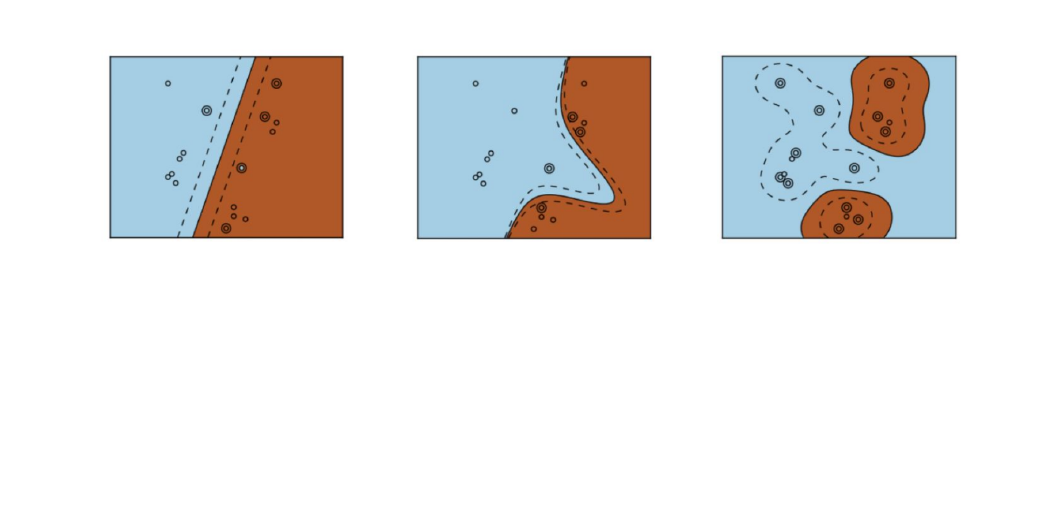
\includegraphics[scale=0.7]{images/11_6.png}
\end{center}

На картике слева разделяющая поверхность для скалярного произведения, по центру для полиномиального ядра, справа для $RBF$.

С различными ядрами мы можем строить различные разделяющие поверхности. Но проблема всё равно остаётся, популярность SVM упала за последние годы, так как чтобы подобрать ядро в таком алгоритме нужно перебрать возможные ядра, а возможные ядра подобрать <<экспертным мнением>>. Тем более если у нас много задач, в каждой из которых своя выборка, то каждый раз придётся проделывать одну и ту же работу. 



\section{Principal component analysis. Relations to SVD. Eckart-Young theorem. How to apply PCA in practice.}
Метод главных компонент во всех библиотечных реализациях называется РСА, существует для понижения размерности.

\textbf{Мотивация}\\

Вспомним зачем вообще интересно понижать размерность.
\begin{enumerate}
    \item В задачах ML размерность данных может быть очень большой. Например, миллионы признаков, особенно когда это разреженные признаки - становится сложно работать.
    \item Такие данные сложно визуализировать, сложно обучать модели.
    \item Чтобы снизить размерность, нам требуется использовать какой-то механизм, который по-хорошему все-таки воспроизводим.
\end{enumerate}


РСА - линейный способ понижения размерности, который интуитивен и используется широко на практике. Зачем нам может понадобиться матричное разложение на практике?
Матрица объект-признак $X$ может быть приближена произведением двух матриц меньшего ранга:

$$X_{l,d} \approx U_{l, k}V_{k,d}^T$$

Где размерность $k < d, l$. В таком случае мы можем сказать, что у нас есть матрица перехода и матрица, которая кодирует всю информацию. И теперь использовать приближение меньшего ранга для всех наших данных, потеряв часть информации, но используя меньше признаков. \\

Такое разложение можно построить с помощью минимизации $\|X - UV^T\| \to \min$. (Тут норма или норма Фробениуса, или какая-нибудь еще).\
РСА нам говорит, что мы можем матрицу признаков разложить на произведение трех матриц: $X = U\Sigma V^T$.

В этом выражении матрицы $U, V^T$ являются ортогональными матрицами, а $\Sigma$ - диагональная матрица. Можем сказать, что $k$ ненулевых признаков остаются ненулевыми и значимыми. Получаем это с помощью взятия $k$ диагональных элементов матрицы $X$ и соответствующих им столбцов в матрицах $U, V$. Таким образом при перемножении получается итоговая матрица меньшей размерности, итоговый ранг равен $k$.

\begin{center}
    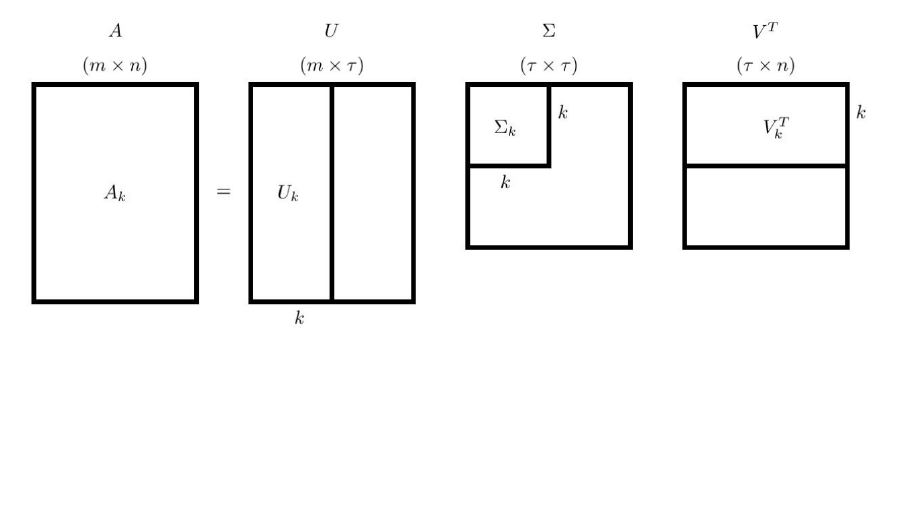
\includegraphics[scale=0.7]{images/12_1.png}
\end{center}

\begin{theorem}[Эскарта-Янга]
$SVD$ дает наилучшую аппроксимацию нашей изначальной матрицы

$$X_k = U_k\Sigma_k V_k^T$$
$$\forall B_k : \rk(B_k) = k$$
$$\|X - B_k\|_F \geqslant \|X - X_k\|_F$$
Где $B_k$ -- матрица ранга $k$, полученная не по SVD разложению.
\end{theorem}

\textit{Плюсы:}

\begin{enumerate}
    \item Так как используемые отображения линейны, значит и РСА - линейная модель, а значит будет работать достаточно быстро
    \item преобразование, из которого можно будет вернуться в исходное пространство, пусть и с какими-то потерями (перешли в другое пространство с помощью $U_k\Sigma_k$, вернулись с помощью $V_k^T$).
\end{enumerate}

Так как у нас матрицы $U, V$ ортогональны, давайте перетасуем все величины на диагонали матрицы $\Sigma$ таким образом, чтобы они шли по убыванию. Первые $k$ элементов -- самые большие величины, которые позволяют описать данные наилучшим способом в $k$-мерном пространстве с точки зрения нормы Фробениуса. \\

\textbf{Интуитивная интерпретация PCA}\\

Представим себе облако точек. 

\begin{center}
    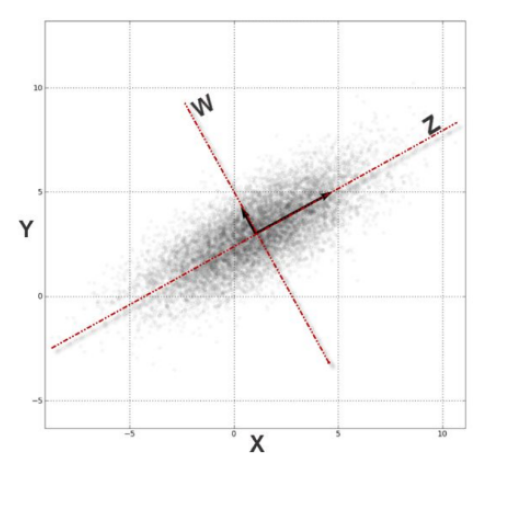
\includegraphics[scale=0.7]{images/12_2.png}
\end{center}

По сути мы переходим в базис главных компонент, которые можно заметить интуитивно: первая главная компонента - вдоль которой дисперсия максимальна (большая ось эллипса, определяем с точностью до направления), вторая и последующие главные компоненты будут ортогональны первой главной компоненте (так как мы помним, что компоненты матрицы ортогональны). \\

Мы работали на картинке в двумерном пространстве, получили две главные компоненты, теперь если мы захотим снизить размерность пространства, нам надо будет выбрать первую главную компоненту, чтобы не потерять максимальное количество информации.\\

\begin{note}
\textit{Вопрос, который любят задавать на собеседованиях:}
Каждая новая компонента смотрит в направлении максимальной дисперсии в оставшемся подпространстве, в котором мы теперь работаем. Все векторы ортогональны друг другу.
Когда РСА выдаёт нам с ошибкой главные компоненты?\\


Понятно, что с точностью до направления они и так неоднозначно могут быть определены, но если у нас есть симметричность в данных - например, они лежат на поверхности сферы, тогда главные компоненты могут быть любые. То есть мы берем любые $k$ ортогональных векторов, где $k$ -- размерность пространства.
\end{note}

\begin{example}[Проблема]
Как правило данные к нам приходят вообще из разных источников. Например, в выборке могут быть признаки: рост, вес, зарплата в долларах, зарплата в рублях и ещё $50$ разных признаков. И мы можем обнаружить, что различные величины находятся в различных шкалах. Допустим рост в см от $50$ до $200$, вес от $40$ до $140$, а зарплата от $10$ до $10000$ в долларах и тд. Тогда получается, что чем больше разброс у того или иного признака, тем больше вдоль этого направления будет дисперсия, тем больше он на себя будет оттягивать внимания у каждой следующей главной компоненты. Это неправильно, так как вместо того, чтобы смотреть на линейные подрпространства и искать информативные комбинации исходных признаков, мы будем смотреть на признаки с большей дисперсией в используемых шкалах.
\end{example}

\begin{note}[Важно]
В принципе проблема та же, с которой мы боролись $L_2$-регуляризацией. Чем больше разброс какого-то признака, тем меньше нам нужны веса для того чтобы моделировать поведение нашей модели. Поэтому если не нормировать данные перед РСА, РСА не даст адекватный результат.
\end{note}

Повторим, что шаг $X_k = U_k \Sigma_k$ даёт понижение размерности, а шаг $\overline{X} = X_kV_k^T$ возвращает нас в исходное пространство.

В принципе, нам может быть интересно посмотреть на отклонение $\overline{X}$ от $X$.

\begin{example}
    Рассмотрим:
    \begin{center}
    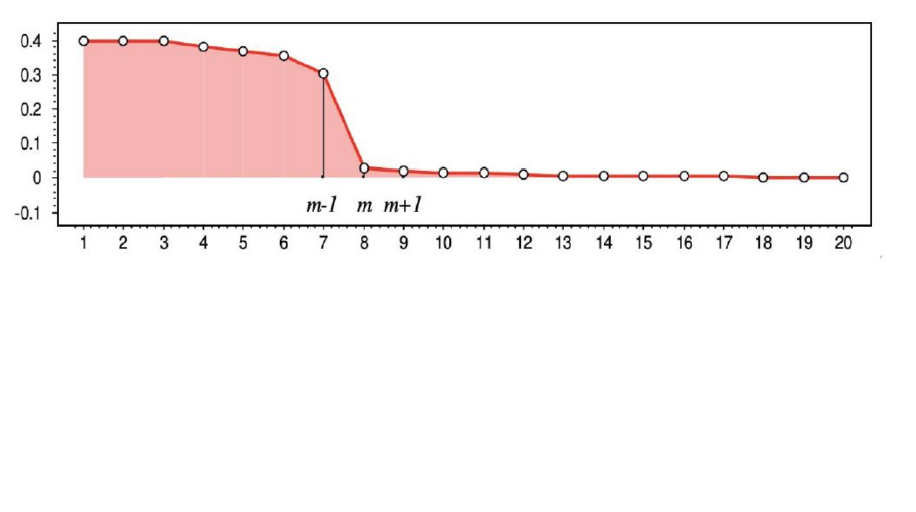
\includegraphics[scale=0.7]{images/12_3.png}
    \end{center}

    В какой-то момент количество дисперсий значительно падает, это значит, что мы нашли линейное подпространство, которое описывает $99\%$ наших данных. И, на самом деле, это как раз то количество главных компонент, которые нужно использовать.
\end{example}

Собственно, на практике мы сначала строим $PCA$ такой же размерности, как и наше пространство (или как максимальное число компонент, которые вообще чисто физически возможно взять). Дальше смотрим на график как из примера выше и уже берем только нужное нам количество.



\section{Train, validation and test stages of model development. Overfitting problem, ways to detect it.}
Для работы модели нужно определить ее гиперпараметры. Рассмотрим две идеи: 

Первая идея (Train, validation and test stage, метод отложенной выборки): обучить модель по части train и по предсказаниям на второй части определить оптимальные гиперпараметры. Минус такого подхода в том, что модель будет зависить от случайного выбора части train (а вдруг объекты в train упорядочены по алфавиту и не все объекты попадут в обучающую выборку при определении гиперпараметров. Модель с этими гиперпараметрами может показать плохой результат на всей обучающей выборке).

Вторая идея (кросс-валидация): часть объектов идет на валидацию, часть на train, затем
данный процесс повторяется несколько раз (часть с валидацией меняется). Тогда мы можем измерить
дисперсию ошибки для каждого набора гиперпараметров и сам лосс, чтобы выбрать оптимальный набор гиперпараметров.

\textbf{Подробнее про Train, validation and test stage:}

\begin{figure}[h]
\centering
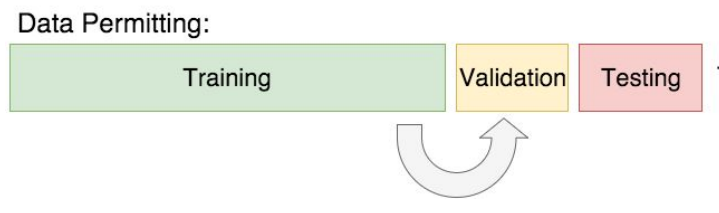
\includegraphics[width=0.5\linewidth]{13.4.PNG}
\caption{Train, validation and test.}
\end{figure}

\textit{Тренировочная выборка} - часть полной выборки, на котором мы обучаем модель. 

\textit{Валидационная выборка} - часть полной выборки, происходит настройка гиперпараметров. Это мы и назовём валидированием или валидацией модели. Изначально человек из каких-то знаний, опыта и других соображений выбирает некоторый пул гиперпараметров для текущей задачи. И далее по ним с каким-то шагом запускаем модель и проверяем получившиеся
предсказания с помощью метрик качества модели. Выбирает и фиксирует значения гиперпараметров.

\textit{Тестовая выборка} - часть полной выборки, который мы заранее отложили и проверяем значение функции потерь, а также метрики качества модели.
НЕ НАДО ВАЛИДИРОВАТЬСЯ НА ТЕСТОВОЙ ВЫБОРКЕ. Считайте, что проверка на тестовой выборке - это как финальная проверка работы. Уже с оптимизированными параметрами и гиперапараметрами запускаем модель, чтобы проверить её качество на этой части данных. Иногда для конечного теста, в тестовую выборку докидывают и валидационный датасет, но такой шаг является спорным.

\textbf{Overfitting problem, ways to detect it.}

\textbf{Определение.} Недообучение — ситуация, когда модель уловила не все общие закономерности и не способна достаточно точно воспроизвести распределение, из которого создаются объекты. Недообучение связано с тем, что по каким-то причинам алгоритм не уловил закономерностей в данных. Это явление, обратное переобучению, при котором алгоритм не полностью использует предоставленные ему для обучения данные.

\textbf{Определение.} Переобучение — ситуация, когда модель не только успешно смоделировала распределение, но и включила в него шумовые факторы (то есть переобучилась под выбросы). То есть построенная модель хорошо работает на объектах из тестовой выборки, но плохо работает на объектах, не участвовавших в тестовой выборке.

\begin{figure}[h]
\centering
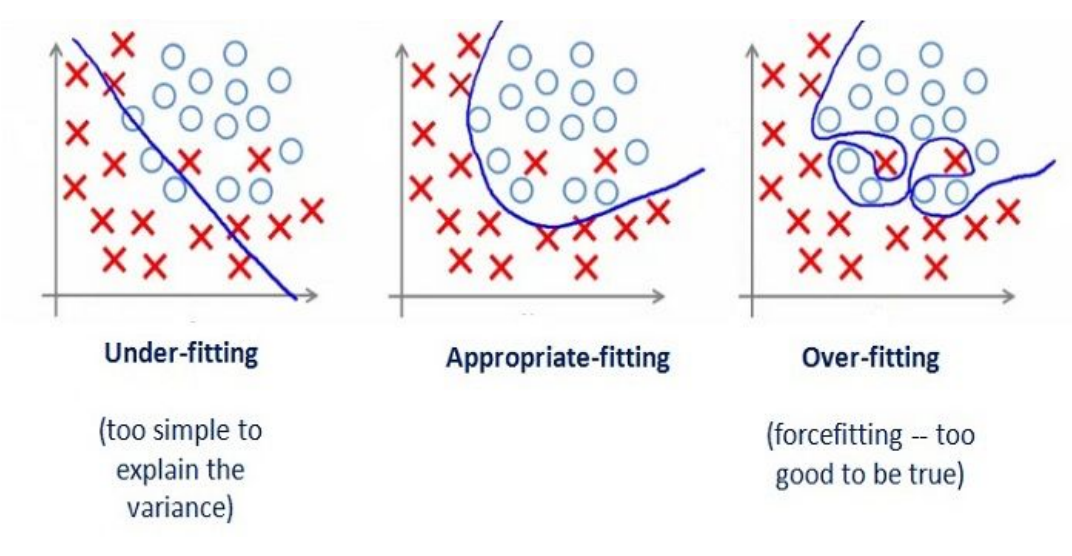
\includegraphics[width=0.6\linewidth]{13.1.PNG}
\caption{Недообучение, хороший фит, переобучение.}
\end{figure}

\textbf{Как детектировать это все?}

Вспомним про train и test, будем измерять лосс на них в зависимости от сложности модели (например,
число эпох или норма вектора весов в линейной регрессии).

• Если и на train, и на test лосс падает, то мы уловили не все основополагающие зависимости
$\Longrightarrow$ недообучение.

• Если на train лосс падает, а на test лосс растет, то мы уловили шумовые зависимости, чуждые
распределению $\Longrightarrow$ переобучение

Подробнее разберём вопрос: переобучение и недообучение. Когда мы просто запоминаем точки из тренировочной выборки, у нас будет не модель, которая будет возможно проходить через все точки на train, но на реальных данных показывать плохие результаты, модель скорее всего будет слишком сложной. А также если наша модель недообучилась, то будет слишком простая, неподходящая под реальность модель. Чем больше мы увеличиваем сложность моделей, тем больше данных нам нужно, чтобы её пофитить, но тем больше у нас возможностей изучить сложные закономерности. Чтобы баланс не нарушить, то есть иметь оптимальное обучение без недообучения и переобучения, нам нужно соблюдать все 3 этапа жизненного цикла построения модели (следует из bias variance decomposition). Оптимальной сложностью или временем обучения нейросети, является тот момент, когда значение функции потерь на валидационной выборке начинает расти при падении значения функции потерь на тренировочной выборке. Хорошо это понять можно по картинке ниже или при построении подобных графиков в реальной жизни - на следующем рисунке обучения бинарного классификатора. 


\begin{figure}[h]
\centering
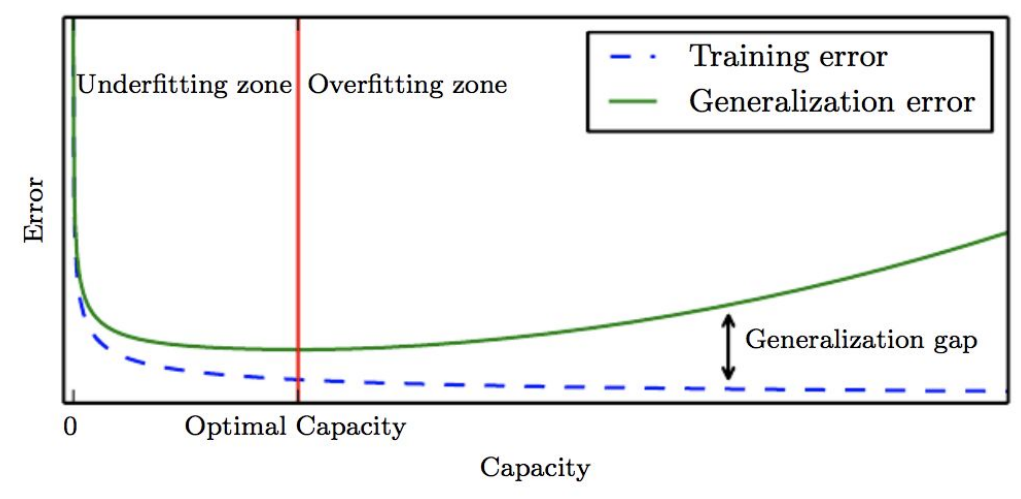
\includegraphics[width=0.5\linewidth]{13.2.PNG}
\caption{Зелёной линией отмечено значение loss function на валидационной выборке, синей линией - на тренировочной. По оси x отмечена сложность модели (эпохи обучения). Красной линией отмечена оптимальная сложность: левее неё недообучение, правее - переобучение.}
\end{figure}

\begin{figure}[h]
\centering
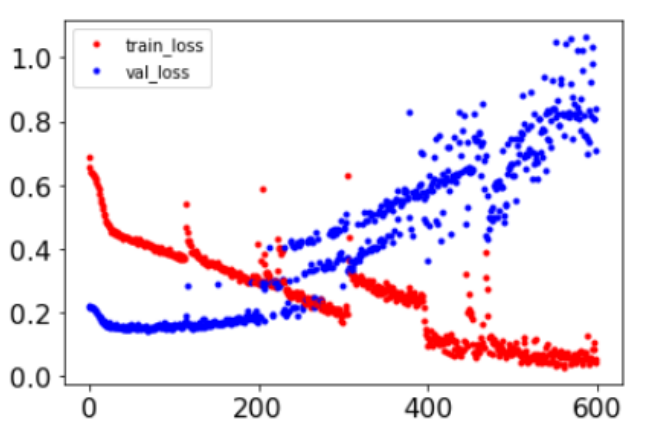
\includegraphics[width=0.4\linewidth]{13.3.PNG}
\caption{Поведение функции потерь бинарного классификатора на валидационной и тренировочной выборке от эпохи обучения нейросети.}
\end{figure}

То есть переобучение - это когда значение функции потерь на валидационной выборке растёт, а на тренировочной падает. Недообучение - когда они все вместе убывают и ещё не надо останавливаться в обучении.



\section{Validation strategies. Cross validation. Data leaks.} 
Вернёмся к идее кросс-валидации:

\textit{Кросс-валидация} - это когда мы делим выборку на k кусочков, на k-1 используем как train, 1ый кусочек используем как валидацию. Потом берём второй кусочек, на остальных обучаемся и предсказываем на 2ом. И так проходимся по всем k кусочкам, то есть потребуется построить k моделей, тогда появится предсказание для каждого значения. В результате получается оценка эффективности выбранной модели с наиболее равномерным использованием имеющихся данных.

\begin{figure}[h]
\centering
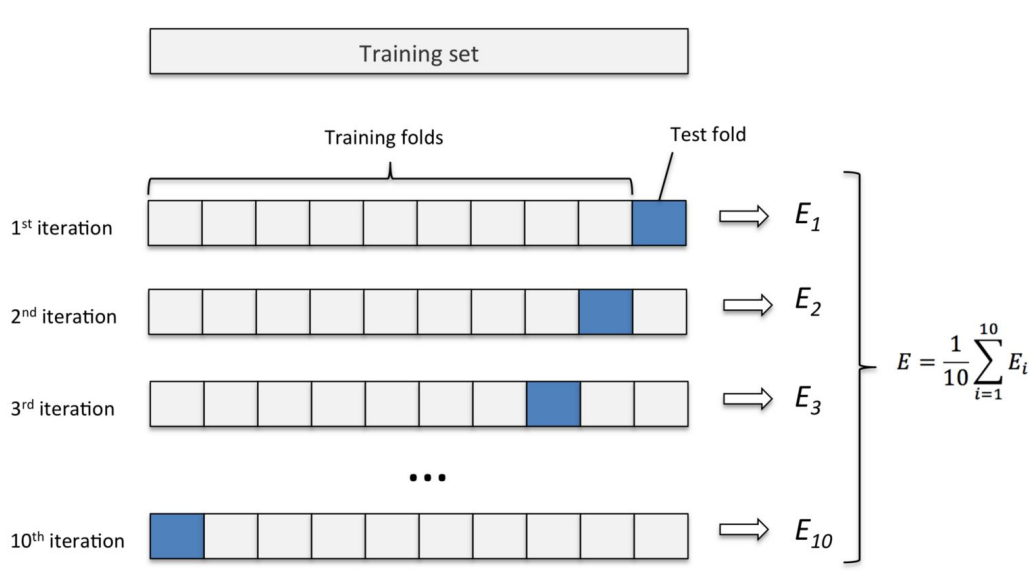
\includegraphics[width=0.5\linewidth]{14.1.PNG}
\caption{}
\end{figure}

Не путать кросс-валидацию и валидацию в целом.

Как соотносятся размеры тренировочной и валидационной выборки?(Вопрос из зала)

От 90/10 до 70/30, зависит от задачи и колиества данных. 

Note. Далее речь идет о K-fold кросс-валидации, где K — число запусков кросс-валидации и одновременно то, на сколько примерно равных кусков мы бьем train. 

Тогда в рамках каждого запуска один из K блоков является валидацией, а остальные — train.

Влияние количества блоков:

• При увеличении числа блоков дисперсия ответа уменьшается (закономерно, поскольку объем данных
увеличивается)

• Аналогичная ситуация с bias - матожидание разности между истинным ответом и выданным
алгоритмом - оно уменьшается.

• Чем меньше количество блоков, тем быстрее это работает, но тем меньше шанс, что модель
подстроится под какой-то кусок данных.

Кросс-валидацию следует делать, когда данных мало, потому что она работает лучше. Но, когда выборки огромные, делать кросс-валидацию очень долго. Используем Train, validation and test stage поскольку количество данных и так позволяет хорошо обучить модель.

\textit{Data leak} - утечка данных, при которой обучение происходит в том числе и на тестовых данных.


\section{Bias-variance tradeoff.}
\textbf{Прим.} Билет взят из открытых источников: \href{https://towardsdatascience.com/understanding-the-bias-variance-tradeoff-165e6942b229}{1} \href{https://en.wikipedia.org/wiki/Bias%E2%80%93variance_tradeoff#:~:text=The%20bias%E2%80%93variance%20decomposition%20is,noise%20in%20the%20problem%20itself.}{2} (тема не найдена на лекциях)
\\

Цель билета - рассказать о проблеме поиска балланс между недообучением и переобучением.

\textit{Компромисс между смещением и дисперсией} - это свойство набора моделей предсказания, когда модели с меньшим отклонением (low bias) от имеющихся данных имеют более высокую дисперсию (high variance) на новых данных (то есть подвержены переобучению), и наоборот модели с меньшей дисперсией (low variance) от имеющихся данных имеют более высокое смещение (high bias) на новых данных (это приводит к недообучению). Ниже более подробное объяснение этого процесса. Возникает конфликт при попытке одновременно минимизировать эти два источника ошибок, которые мешают алгоритмам обучения с учителем делать обобщение за пределами тренировочного набора.

Смещение - это разница между средним прогнозом нашей модели и правильным значением, которое мы пытаемся предсказать. Модель с высоким смещением уделяет очень мало внимания данным обучения и чрезмерно упрощает модель. Это всегда приводит к высокой погрешности в обучающих и тестовых данных. (недообучение).

Дисперсия - это изменчивость прогноза модели для данной точки данных или значения, которое говорит нам о разбросе наших данных. Модель с высокой дисперсией уделяет большое внимание обучающим данным и не обобщается на данные, которые она раньше не видела. В результате такие модели очень хорошо работают с обучающими данными, но имеют высокую частоту ошибок в тестовых данных. (переобучение)
\\
\textbf{Математическое обоснование}

Пусть переменная, которую мы пытаемся предсказать, равна $Y$, а другие ковариаты - $X$. Мы предполагаем, что между ними существует такая взаимосвязь, что
$Y=f(X) + e$. Где $e$ - член ошибки, и он обычно имеет матожидание 0.

Мы создадим модель $\hat{f}(X)$, используя линейную регрессию или любой другой метод моделирования.
Таким образом, ожидаемая квадратическая ошибка в точке $x$ равна

$$Err(x) = \mathbb{E}[(Y - \hat{f}(x))^2]$$

Можно разложить в:

$$Err(x) = (\mathbb{E}[\hat{f}(x)] - f(x))^2 + \mathbb{E}[(\hat{f}(x) - \mathbb{E}[\hat{f}(x)])^2] + \sigma^2_{e}$$
$$Err(x) = Bias^2 + Variance + Irreducible Error$$

$Err(x)$ - это сумма смещения$^2$, дисперсии и неустранимой ошибки.

Неустранимая ошибка - это ошибка, которую нельзя уменьшить путем создания хороших моделей. Это показатель количества шума в наших данных.

\begin{figure}[h]
\centering
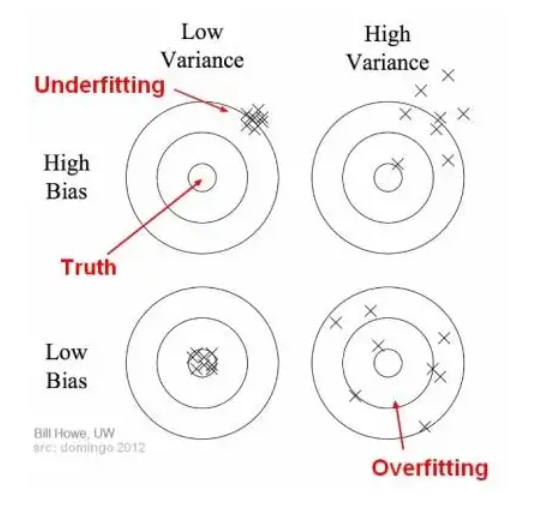
\includegraphics[width=0.4\linewidth]{15.1.PNG}
\caption{Расположение тестовой выборки относительно модели.}
\end{figure}
\\
\textbf{Проблема Bias-Variance Tradeoff}

Это проблема сравнения $Bias^2$ vs. $Variance$. Если наша модель слишком проста и имеет очень мало параметров, она всего будет иметь большое смещение и низкую дисперсию. С другой стороны, если наша модель имеет большое количество параметров, она будет иметь высокую дисперсию и низкое смещение. Поэтому нам нужно найти правильный/хороший баланс без переобучения и недообучения данных. Для этого, нам нужно найти хороший баланс между смещением и дисперсией таким образом, чтобы свести к минимуму общую ошибку.

$$TotalError = Bias^2 + Variance + Irreducible Error$$

\begin{figure}[H]
\centering
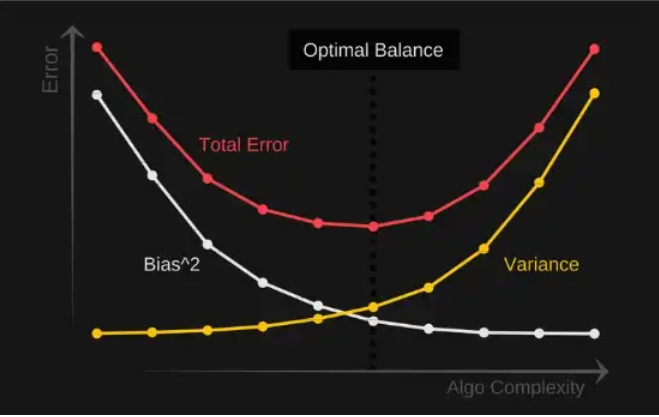
\includegraphics[width=0.4\linewidth]{15.2.PNG}
\caption{}
\end{figure}

\section{Decision tree construction procedure.}
\textbf{Решающие деревья.} 

\begin{figure}[H]
\centering
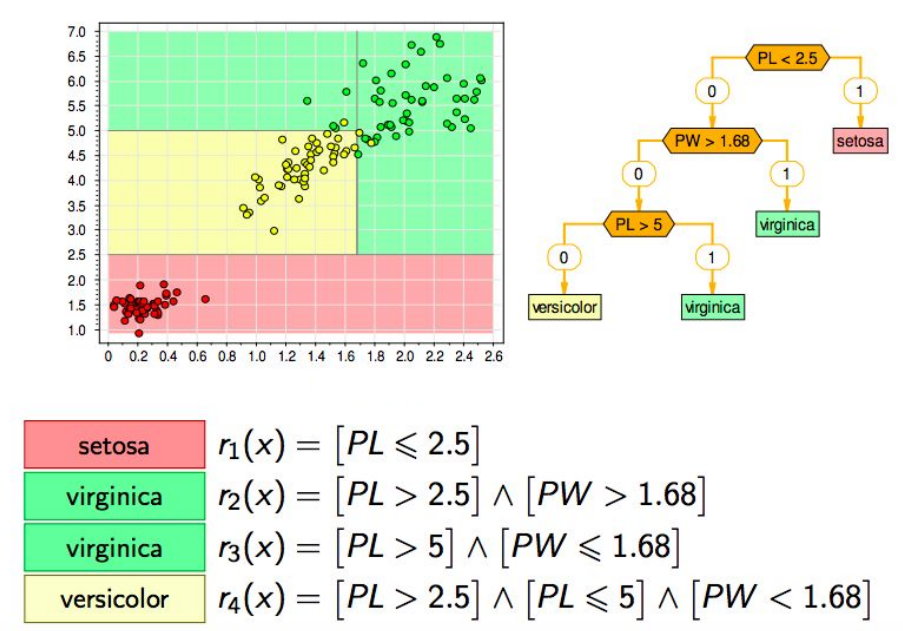
\includegraphics[width=0.5\linewidth]{16.1.PNG}
\caption{Датасет Ирисы Фишера и классификатор в виде дерева.}
\end{figure}

Поговорим об интуиции, лежащей под капотом решающего дерева. Давайте взглянем на знакомый датасет Ирисы Фишера. На рисунке ниже можем увидеть алгоритм классификации в виде дерева, который на каждом шаге использует предикат и с помощью этого делает какое-то решение одно из двух. Делаем на первом шаге разделение на два листа по значению 1го признака. В первый класс попали все объекты класса setosa, в нулевой класс всё остальное. Теперь по значению второго признаку, мы делим оставшуюся часть пространства пополам. Всё, что попало в класс 1 - virginica, в класс 0 остались зелёные и жёлтые признаки. Следующий шаг опять в делении по уже другому трешхолду 1го признака на две выборки, в одной из них virginica, в другой желтый versicolor. На рисунке дерево глубины 3, но некоторые объекты проклассифицировались неправильно,
поэтому мы можем достроить дерево более глубоким, чтобы все точки были проклассифицированы правильно. С одной стороны было бы хорошо так точно угадывать класс, но с другой стороны мы получим очень глубокое, то есть переобученное дерево. Так как мы пытаемся уловить возможно шумовые наблюдения в нашей обучающей выборке, мы переобучаемся под неё и теряем общую идею, которую мы могли бы перенести в тестовую выборку. Если присмотреться к такому классификатору, можно заметить, что каждому подпространству модель предсказывает константу. Если посмотреть на задачу регрессии на рисунке ниже, это видно ещё лучше. Тут изображён синус, который зашумлен и мы пытаемся описать эту гладкую функцию с помощью решающего дерева. В данном случае признаковое пространство 1мерное. Получается кусочно-постоянная функция. Потому что мы делим

\begin{figure}[h]
\centering
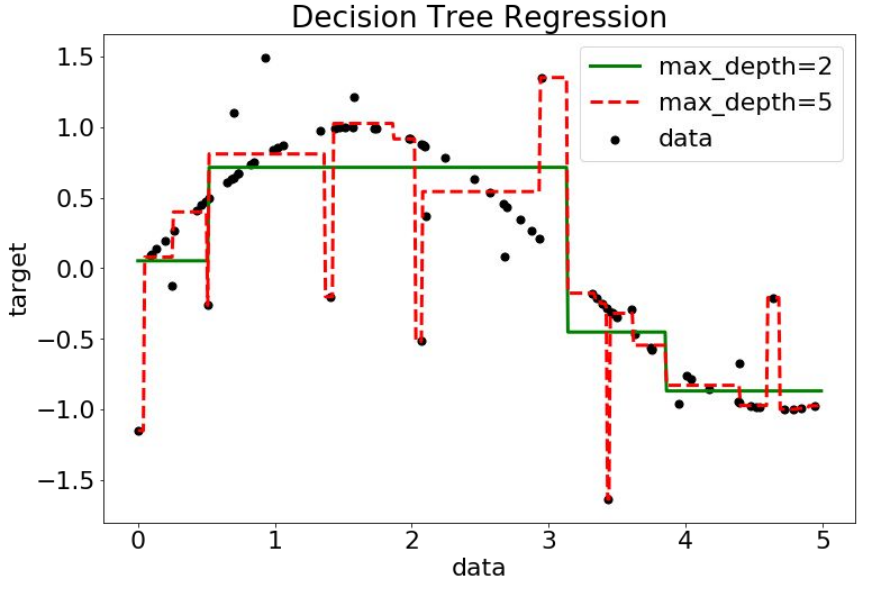
\includegraphics[width=0.5\linewidth]{16.2.PNG}
\caption{Решающие деревья в задаче регрессии.}
\end{figure}

признаковое пространство на куски и каждому куску сопоставляем некоторую константу. Красным показано дерево глубины 5, а зелёным - глубины 2. Мы видим, что красное дерево поймало шумовые точки - переобучилось. Так получилось, потому что на этих точках была большая ошибка, дерево пыталось минимизировать
ошибку и добилось такого фита. Дерево глубины 2 не очень хорошо описывает синус, но оно не переобучилось. Как нам построить дерево, а не просто применить построенное? Для этого нам требуется поставить оптимизационную задачу и обсудить как можно работать с деревом.

5.1 Построение модели решающего дерева

Сразу можно заметить, что поскольку функция, которую строит дерево кусочно-постоянная, а значит градиентные методы работать не будут (в каждом месте, где происходит разрыв, производная вообще не будет
определена). Нам придётся вернуться к жадной оптимизации за неимением лучшего метода.
\begin{enumerate}
    \item Пусть $x^{(j)}$ - $j$-ый признак
$$x^{(j)} < t$$

В данный момент времени мы находимся в ноде дерева, и в ней мы делим все объекты по j-ому признаку,
сравнивая его с трешхолдом t. Если признак у объекта меньше t, то объект идёт в левое поддерево, если
больше - в правое поддерево. Получаются две новые ноды (это левое и правое поддерево).
    \item  Делаем тоже самое для каждой новой ноды. Рекурсивный алгоритм.
\end{enumerate}


Откуда брать трешхолд и порог по индексу?

Поскольку датасает имеет конечное число признаков, которыми он описывается, то можно перебрать только конечное число трешхолдов, так как объектов тоже ограниченное количество. То есть будет 2 вложенных цикла: перебираем все возможные признаки, и все возможные трешхолды. 

Нам нужен формальный критерий, по которому мы можем понять насколько качественное разбиение. 

\begin{figure}[h]
\centering
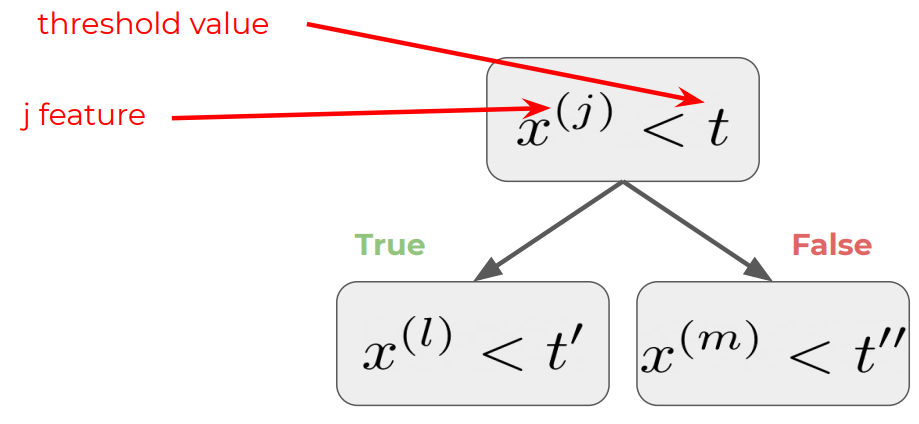
\includegraphics[width=0.5\linewidth]{16.3.PNG}
\caption{Иллюстрация разбиения в ноде.}
\end{figure} 

Пусть текущее условие $x^{(j)} < t$ действует в области $Q$. Условие  делит пространство $Q$ на две части $L$ и $R$. Введём функцию $G$ - взвешенную сумму функции информативности от левой, правой подвыборок:
$$G(j, t) = \frac{L}{Q} H(L) + \frac{R}{Q} H(R)$$
Логично, что в сумма $\frac{L}{Q} + \frac{R}{Q} = 1$.
$G(j, t)$ - указывает на то, насколько разбиение по $t$ является хорошим для нас. Чем значение больше, тем лучше.

Будем помнить, что дерево даёт только константу для каждого из листов (Это области, которые алгоритм не стал делить). Посмотрим на рисунок ниже. Для этого надо посчитать выборочные вероятности для классов встречающихся объектов в листе и выбрать наибольшую сумму.

\begin{figure}[h]
\centering
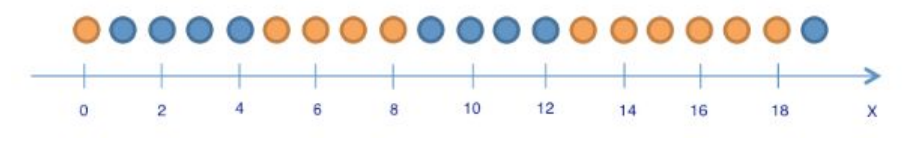
\includegraphics[width=0.5\linewidth]{16.4.PNG}
\caption{Классификация по 1 признаку.}
\end{figure}

Есть задание простое задание классифицировать шарики. Признак - одно число. И два класса.



Если нам надо разделить на 2 признака выборку по какой-то границе, то скорее всего мы обрежем так, чтобы с одной стороны доминировал один класс, а с другой - другой.

Обратите внимание на картинку ниже. Введём понятие упорядоченности или информационного критерия H(R). Под упорядоченностью понимается то, насколько сложно будет описать выборку, которая попала в лист. В простейшем случае бинарной классификации мы имеем дело с misclassification criteria:
$H(R) = 1 - max\{p_0, p_1\}$, где $p_0$ - доля значений класса 0 в выборке $R$, $p_1$ - доля класса 1 в выборке $R$. $p_0 + p_1 = 1$. 

\begin{figure}[h]
\centering
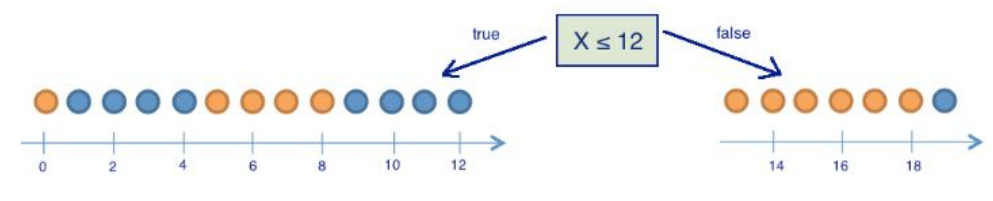
\includegraphics[width=0.5\linewidth]{16.5.PNG}
\caption{Разбиение на 2 подвыборки.}
\end{figure}

Оценивает 1 - выборочную вероятность данного класса. То есть по сути это вероятность ошибиться, если мы предсказываем самый доминирующий класс. Не очень хороший подход, потому что он игнорирует все недоминирующие классы, для многоклассовой классификации это плохо. Такой критерий приведен скорее для исторической справки. Нам важны следующие 2 критерия:
\begin{enumerate}
    \item  Entropy criteria:
$$H(R) = -p_0 \log p_0 - p_1 \log p_1 $$
    \item  Gini impurity:
$$H(R) = 1 - p_0^2 - p_1^2 = 1 - 2p_0p_1 $$
\end{enumerate}

Деревья, как и Наивный Байес работают с классификацией одинаково, вне зависимости от количества классов.

\section{Information criteria. Entropy criteria, Giny impurity.}
Хотим построить лист $x^{(j)} < t$. Хотим ввести какую-то характерестику <<гетерогенности>> $H$ и мимнимизировать выражение 

\[ \frac{|L|}{|Q|} H(L) + \frac{|R|}{|Q|} H(R) \rightarrow min_{j, t},\]

где $Q$ - множество, которое разбивается этим листом, а $L, R$ - части, на которое оно разбивается

Более простым языком: $H$ - показывает насколько сильный разброс данных в этом множестве (чем он меньше, тем ближе все данные будут к предсказанному значению).

\begin{definition}
    Функция $H$ называется \textit{критерием информативности} (information criteria)
\end{definition}

Есть разные способы задать $H$ для задачи классификации. Посмотрим сначала на примере бинарной классификации. Далее $p_i$ - нормированная частота встречаемости $i$-ого класса в множестве $R$

\begin{enumerate}
    \item Misclassification criteria: количество ошибок классфикации (предсказываем доминирующий класс и смотрим сколько объектов классифицировали неправильно)

    \[ H(R) = 1 - \max\{p_0, p_1\}\]

    Не очень хороший способ: например для многоклассовой классификации дерево может хорошо отделять несколько каких-то классов от остальных, но этот критерий нам этого не покажет

    \item Entropy criteria

    \[ H(R)=-p_0 \log p_0 - p_1 \log p_1 = -p_0 \log p_0 - (1-p_0) \log (1-p_0)\]

    Энтропия <<на пальцах>>: чем больше энтропия, тем больше хаоса

    \item Gini impurity

    \[ H(R)=1 - p_0^2 - p_1^2 = 1 - p_0^2 - (1-p_0)^2=2p_0 (1- p_0)\]

    Интуитивно: берем два объекта из нашей подвыборки. Какова вероятность, что они окажутся разных классов?
\end{enumerate}

Для многоклассовой классификации аналогично

\begin{enumerate}
    \item Misclassification: $H(R)=1- \max \{ p_0, \ldots, p_k \}$

    \item Entropy: $H(R)=-\sum_{i=0}^k p_i \log p_i$

    \item Gini: $H(R)=1 - \sum_{i=0}^k p_i^2$
\end{enumerate}

\begin{figure}[H]

\centering

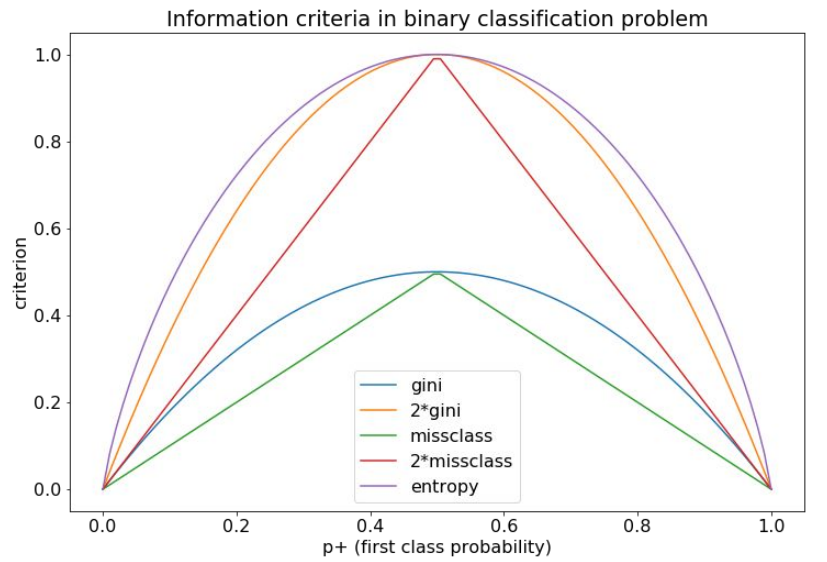
\includegraphics[width=0.6\linewidth]{images/information criteria.png}

\caption{График разных критериев информативности}

\end{figure}

Из графика выше видим, что энтропия и Джини ведут себя примерно одинаково и на практике не очень отличаются (вроде в последнее время чаще используют Джини). Так же график показывает, что misclassification слишком мало штрафует за малые ошибки (по сравнению с остальными критериями)

Для задачи регрессии нам придется взять другой критерий информативности (mean squared error)

\[ H(R) = \min_c \frac 1 {|R|} \sum_{(x_i, y_i) \in R} (y_i - c)^2\]

Оптимальная константа (оценка максимального правдоподобия на $c$): 

\[ c^*=\frac 1 {|R|} \sum_{y_i \in R} y_i \]

Интуитивно: считаем дисперсию относительно среднего

Вопрос <<со звёздочкой>>: если оптимизируем MAE, то $c^*$ --- это медиана

Подробнее про то, почему получаются такие оценки можно почитать \href{https://d18ky98rnyall9.cloudfront.net/rpPnDwIOSFaT5w8CDnhWWA_44e3f19ed9fd4e56baa1c8ce9ba064b5_loss_functions.pdf?Expires=1673308800&Signature=Bpev8rp2H1yc4cLEgoHJVJyO~3J-4z0SR9hTDea8xAZfKECVNgdr7bG~N33xj71vSyGs8jOkXWwZKRw-q2x5wTxxQDPsiV7K71MAItbktK83ranmPjApYcBipi9rimYRQAoLwKOBZr5RtF0DEiF7FXr5HaBuh4KXCQMnOYSqoFs_&Key-Pair-Id=APKAJLTNE6QMUY6HBC5A}{здесь} 

\section{Ensembling methods. Bootstrap. Bagging.}
Рассмотрим выборку $X$ размера $m$. Выберем $m$ объектов с повторениями из $X$ и получим \textit{бутстрапированную выборку}. Повторим данный процесс $N$ раз чтобы сгенерировать $N$ выборок $X_j$.

Мы сделали это для того, чтобы получить много выборок похожих на $X$, но при этом не совпадающих с ним. 

Возьмем нашу модель. Обучим ее на каждом $X_j$ поотдельности. Введем обозначения

\[ \varepsilon_j(x) = b_j(x)-y(x)\]

\[ \E (b_j(x) - y(x))^2=\E_x \varepsilon_j^2(x)\]

\[ \E_1 = \frac 1 N \sum_{j=1}^N \E_x \varepsilon_j^2(x),\]

где $b_j(x)$ - предсказание модели, обученной на выборке $X_j$, $y(x)$ - истинный ответ для объекта $x$, $\varepsilon_j(x)$ - ошибка $j$-ой модели, $\E_1$ - средняя ошибка всех моделей

Предположим, что ошибки моделей обученных на разных бутстрапированных выборках несмещены и нескоррелированы, т.е.

\[ \E_x \varepsilon_j(x) = 0\]

\[ \E_x \varepsilon_i(x) \varepsilon_j(x)=0, \quad i \neq j\]

Рассмотрим модель, которая усредняет предсказния всех моделей полученных ранее. Обозначим ее предсказание за $a(x)$. Тогда

\[ a(x)=\frac 1 N \sum_{j=1}^N b_j(x)\]

Найдем ошибку этой модели $\E_N$

\[ \E_N = \E_x \left( a(x) - y(x)\right)^2=\E_x \left( \frac 1 N \sum_{j=1}^N b_j(x) - y(x)\right)^2 = \E_x \left(\frac 1 N \sum_{j=1}^N \varepsilon_j(x) \right)^2= \] 

\[ = \frac{1}{N^2} \E_x \left( \sum_{j=1}^N \varepsilon_j^2(x) + \underbrace{\sum_{i \neq j} \varepsilon_i(x) \varepsilon_j(x)}_{=0} \right) = \frac 1 N E_1 \]

Получили, что ошибка упала в $N$ раз. Что мы сделали не так? (если все хорошо, то изобрели какой-то гениальный метод и вся остальная машинка не нужна)

Ответ: предположение о несмещенности и нескоррелированности не всегда верно на практике. 

Попробуем это исправить: с ошибкой каждой конкретной модели мы мало что можем сделать, но можем попробовать сделать так, чтобы ошибки разных моделей были не похожи друг на друга. Это должно уменьшить корреляцию ошибок и соответственно приблизить сумму из равенства выше к 0 и приблизиться к теоретическому результату. Воспользуемся слабостью деревьев: их склонностью к переобучению. Переобучим каждую модель под конкретную бутстрапную выборку, и потом усредним результаты. 

Но бутсрапные выборки все же очень похожи, поэтому это не приведет нас к желаемому результату. Поэтому мы в каждой выборке хотим выбрать признаки, на которых будет обучаться модель. Подробнее об этом поговорим в следующем билете

\begin{definition}
    Прием усреднения предсказаний модели, обученной на разных бутстрапных выборках называется \textit{бэггингом} (bagging = bootstrap aggregation)
\end{definition}

\begin{lemmanote}
    Усреднение по моделям работает только в том случае, если предсказания моделей осмысленны и мы просто хотим уменьшить дисперсию (понятно, что если модели выдают что-то рандомное никакое усреднение нам не поможет)
\end{lemmanote}

\section{Random Forest, Random subspace method.}
\textbf{Random Subspace Method (RSM):} случайно выбираем некоторые наборы признаков, обучаем модель только на них и усредняем результаты. Из-за того, что наборы признаков разные, ошибки не очень похожи друг на друга, а значит мы приближаемся к теоретическому результату из прошлого билета

\textbf{Random Forest:} объединим bagging и RSM на деревьях, чтобы ошибки стали еще менее похожими

Плюсы random forest: нелинейная разделяющая поверхность, сложно переобучить (переобучения всех деревьев усредняются, проблемы могут быть только если возьмем огромное количество деревьев и наборы признаков будут повторяться), не ломается при наличии скоррелированных признаков, деревья хорошо работают с пропусками (если нет признака, который нужен для этого листа, просто считаем значения в каждой из веток и усредняем)

\[ \hat{y} = \frac{|L|}{|Q|} \hat{y_L} + \frac{|R|}{|Q|} \hat{y_R}\]

Так же random forest позволяет использовать обучающую выборку для валидации: так как мы обучаем каждое дерево на бутстрапной выборке, есть объекты, которые каждая из моделей не видела. Поэтому можно для каждого объекта взять только те модели, которые его не видели и усреднить предсказания по ним. Получим оценку сверху на ошибку (так как уменьшили ансамбль, следовательно ошибка выросла).

\[ OOB = \sum_{i=1}^m L\left(y_i, \frac 1 {\sum_{n=1}^N I[x_i \not\in X_n]} \sum_{n=1}^N I[x_i \not\in X_n] b_n(x_i)\right) \quad \text{(out-of-bag error)} \]

\begin{lemmanote}
    Если данные упорядочены во времени надо быть очень осторожными с OOB, потому что важно смотреть распределение <<новое при условии старого>>, а не наоборот (иначе модель обучается чему-то не тому)
\end{lemmanote}
\textbf{Модификации:}
\begin{enumerate}
    \item Extremely Randomized Trees: выбираем разделения в листах более рандомно (в экстремальном случае: деревья даже не зависят от ответов обучающей выборки)

    \item Isolation forest (метод поиска аномалий): не предсказываем что-то, а пытаемся отделить аномалии, так как их проще отделить деревом чем остальные точки (этот метод не универсальный, работает не на всех задачах. Пример: точки на плоскости, <<свернули в рулон>> и добавили аномалии между слоями. Метод будет работать плохо)
\end{enumerate}

\section{Boosting and gradient boosting. Main idea, gradient derivation.}
Идея бустинга: берем несколько последовательных моделей. Каждая следующая предсказывает ошибку предыдущей 

\begin{figure}[H]

\centering

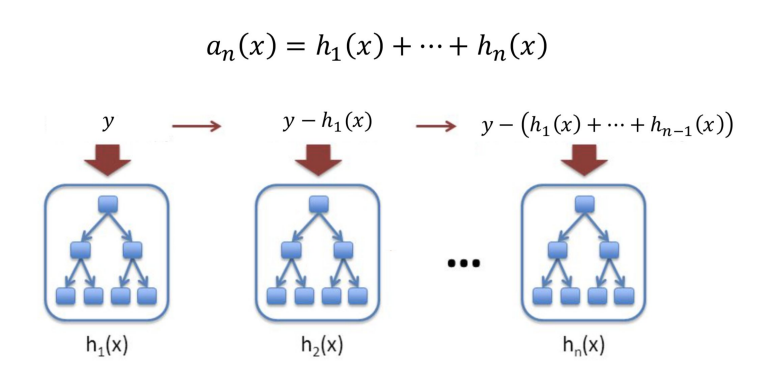
\includegraphics[width=0.8\linewidth]{images/boosting intuition.png}

\end{figure}

\begin{example}
    Рассмотрим игрушечный пример на задаче бинарной классификации (см. картинки ниже). Каждая модель будет <<решающим пнем>> (деревом с одним разделением). После того как обучим все модели с учетом ошибок предыдущих (размер точек показывает ошибку) сложим их с какими-то весами и получим итоговую нелинейную модель
    
    \begin{figure}[H]
    \centering
    \begin{subfigure}
      \centering
      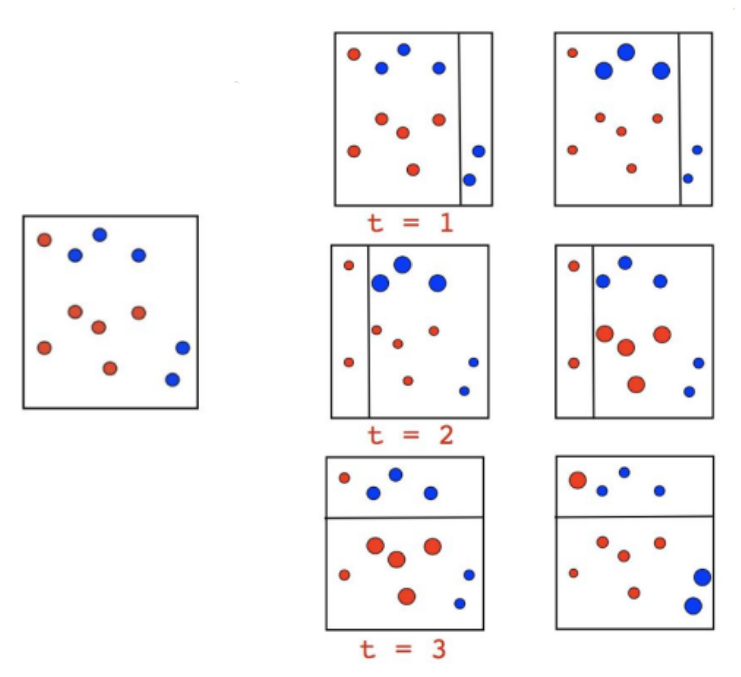
\includegraphics[width=0.4\linewidth]{images/boosting intuition learning.png}
    \end{subfigure}
    \begin{subfigure}
      \centering
      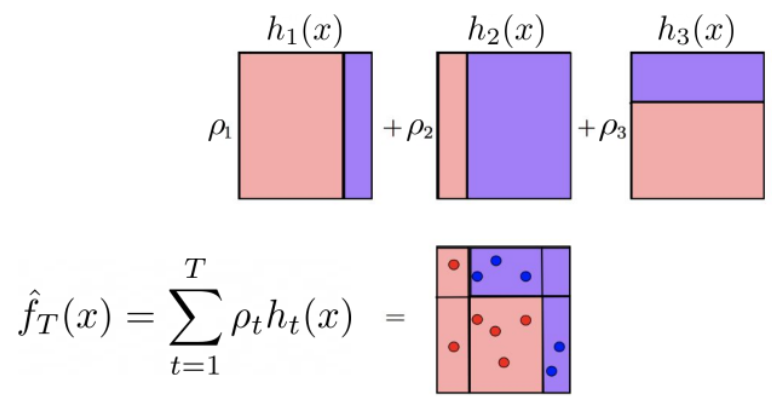
\includegraphics[width=0.4\linewidth]{images/boosting intuition result.png}
    
    \end{subfigure}
    \end{figure}
    
\end{example}

\begin{example}
    Рассмотрим экспоненциальную функцию потерь $E(M)=e^{-M}$. Тогда

    \[ \hat{f}_T = \sum_{t=1}^T \rho_t h_t(x)\]

    \[ L(y_i, \hat{f}_T(x_i)) = \exp (-y_i \hat{f}_T(x_i))=\exp (-y_i \sum_{t=1}^T \rho_t h_t(x_i))=\underbrace{\exp (-y_i \sum_{t=1}^{T-1} \rho_t h_t(x_i))}_{\text{const on step T}} \cdot \exp (-y_i \rho_T h_T(x_i)) =\]
    
    \[=w_i \cdot \exp (-y_i \rho_T h_T(x_i))\]

    Видим, что у каждого объекта есть вес, зависящий от ошибок прошлых моделей, а на шаге $T$ нам нужно минимизирвоать только последнюю функцию. Такой бустинг называется \textit{AdaBoosting} (адаптивный). Однако он был не очень хорош: легко переобучался, экспонента мешала вычислительно и не всегда подходила под задачу
\end{example}

\textbf{Gradient boosting:} идейно мы применяем градиентный спуск в пространстве моделей

Рассмотрим датасет $\{(x_i, y_i)\}_{i=1, \ldots, n}, L(y,f)$ - функция потерь. Тогда оптимальная модель $\hat{f}$ имеет вид

\[ \hat{f}(x)=\argmin_{f(x)} L(y, f(x))=\argmin_{f(x)} \E_{x,y} L(y, f(x))\]

Пусть модель взята из параметрического семейства

\[ \hat{f}(x)=f(x, \hat{\theta})\]

\[ \hat{\theta} = \argmin_\theta \E_{x,y} L(y, f(x, \theta))\]

Рассмотрим шаг индукции: пусть у нас обучены уже $t-1$ последовательных модели. Обозначения:
\[\hat{f}(x) = \sum_{i=0}^{t-1} \hat{f}_i(x)\]

\[ (\rho_t, \theta_t)=\argmin_{\rho, \theta} \E_{x,y} L(y, \hat{f}(x)+\rho \cdot h(x, \theta))\]

\[ \hat{f}_t(x)=\rho_t \cdot h(x, \theta_t)\]

Рассмотрим антиградиент функции ошибки по предсказанию

\[ r_{it} = -\left[ \frac{\partial L(y_i, f(x_i))}{\partial f(x_i)}\right]_{f(x)=\hat{f}(x)}, \quad i=1, \ldots n \]

Настроим нашу следующую модель на предсказание антиградиента

\[ \theta_t = \argmin_\theta \sum_{i=1}^n (r_{it} - h(x_i, \theta))^2 \]

Затем найдем оптимальный шаг в сторону градиента

\[ \rho_t = \argmin_\rho \sum_{i=1}^n L(y_i, \hat{f}(x_i)+\rho \cdot h(x_i, \theta_t)) \]

База индукции: так как каждая следующая модель исправляет ошибку предыдущей нам в принципе неважно с чего начинать, так что можно, например, начать с константы (среднее значение по всему датасету)

Частный случай для линейной регрессии и $L=MSE$

\[ r_{it} = -\left[ \frac{\partial L(y_i, f(x_i))}{\partial f(x_i)}\right]_{f(x)=\hat{f}(x)}=-2(\hat{y}_i - y_i) \]

Получили, что антиградиент пропорционален ошибке, то есть каждая следующая модель напрямую пытается предсказать ошибку предыдущих (в общем случае с другими моделями/функциями потерь это может быть не так)

\begin{lemmanote}
    Важно следить за тем, чтобы градиентный бустинг не переобучился: если переобучится одна модель в цепочке, то все что дальше происходит уже бесполезно. Поэтому если вы пока не понимаете специфику задачи, лучше использовать неглубокие деревья в бустинге (так как их очень сложно переобучить)
\end{lemmanote}

\begin{lemmanote}
    Сам градиентный бустинг не параллелизуется, но так как обычно его делают на деревьев можно распараллелить процесс построения каждого дерева
\end{lemmanote}

\section{Matrix calculus and matrix derivatives. How to get the derivative of matrix/dot product}
\begin{center}
    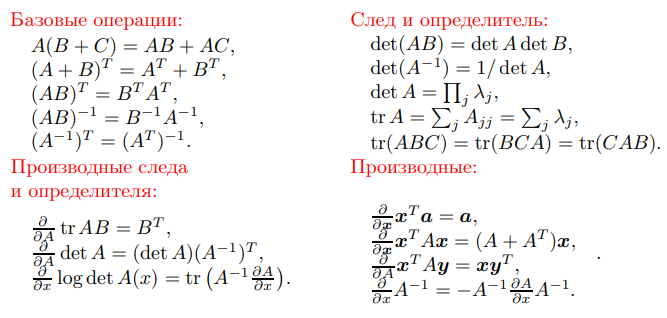
\includegraphics[]{21_1.PNG}
\end{center}
\textbf{Примеры}
\begin{enumerate}
\item
$$  
y = x^Tx,  \quad x \in \mathbb{R}^N 
$$

$$\frac{d}{dx_i} x^T x = \frac{d}{dx_i}  \sum x_i^2 = \frac{d}{dx_i} x_i^2 = 2x_i$$
$$
\frac{dy}{dx} = 2x
$$ 
    \item $$tr(AB) = \sum\limits_{i=1}^n a_{1i}b_{i1} + .... + \sum\limits_{i=1}^n a_{ni}b_{in} \Longrightarrow \frac{dy}{da_{ij}} = b_{ji
}$$
$$
\frac{dy}{dA} = B^T
$$
\item
$$y = a^Tx$$
$$\tfrac{d}{dx_i} a^Tx = \tfrac{d}{dx_i}\sum a_ix_i = a_i \Longrightarrow \tfrac{d}{dx} a^Tx = a$$

\item
$$y = Ax$$
$$\tfrac{d}{dx_i} [Ax]_k = \tfrac{d}{dx_i}\sum_j a_{kj}x_j = a_{kj}$$
$$\tfrac{d}{dx} Ax = A$$
\end{enumerate}


\section{Backpropagation, chain rule.}
\textbf{Chain Rule:}
$$\frac{dL}{dx} = \frac{dL}{dz}\frac{dz}{dx}$$ 
\begin{center}
    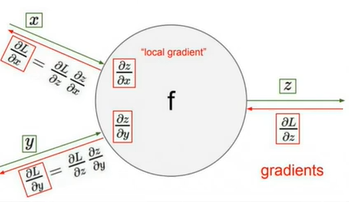
\includegraphics[]{22_1.PNG}
\end{center}
\textbf{BackPropagation} это метод вычисления градиента лосс-функции по параметрам\\

На картинке выше показан шаг BackPropagation для вычисления производной, причем сразу для векторных переменных.

На фазе forward-pass (когда вы пропускаете данные через сеть, умножая на матрицы и прочее), вычисляется выход
вершинки z, который определяется через какую-то функцию, затем вычисляются производные выхода по входам, т.е. $\frac{dz}{dx}$ и $\frac{dz}{dy}$, т.к. все данные для этого у нас есть.
После фазы forward pass’а начинается backward pass, где мы просто применяем Chain Rule на уже вычисленных
производных, вычисляя производные по всем параметрам.
\\

\textbf{Матричная форма}
\begin{center}
    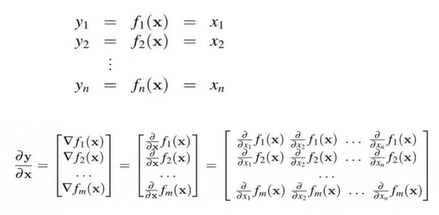
\includegraphics[scale=1.3]{22_3.PNG}
\end{center}

В этом-то умножении (chain rule) и состоит проблема затухания
градиента. Если ваш градиент станет очень маленьким в каком-то месте, то это просто не даст другим градиентам быть не
около 0, т.к. при умножении получается очень маленькое число. В этом случае gradient flow прекращается и сеть перестает
учиться. 

\section{Neural network concept. Fully-Connected layer (FC). Logistic regression as simple NN. XOR problem.}
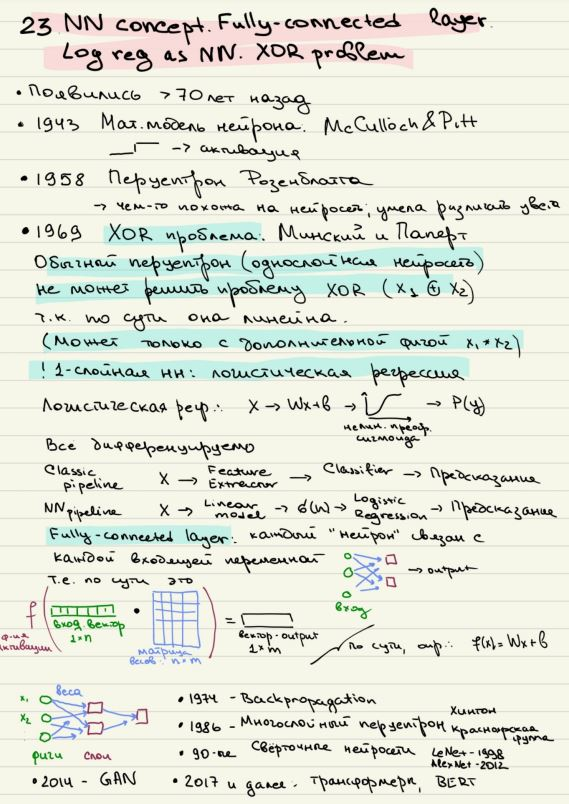
\includegraphics[width=400pt]{images/23.JPG}
\newpage

\section{Losses for NNs: logistic loss, cross-entropy.}
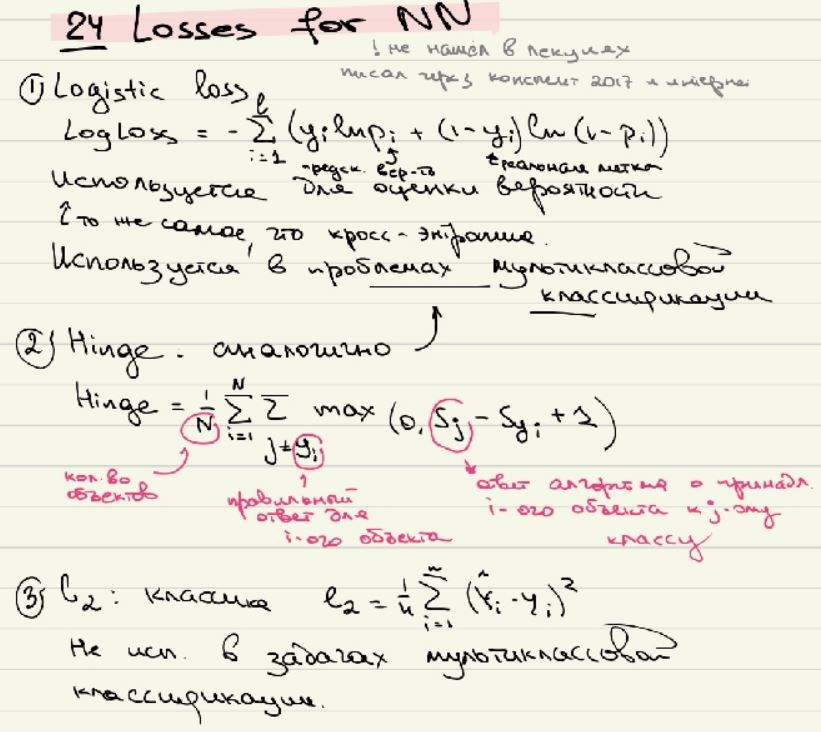
\includegraphics[]{images/24.JPG}
\newpage

\section{Activation functions, their impact on the network, \\ computational complexity. Softmax and LogSoftmax \\ activations, numerical stability.}
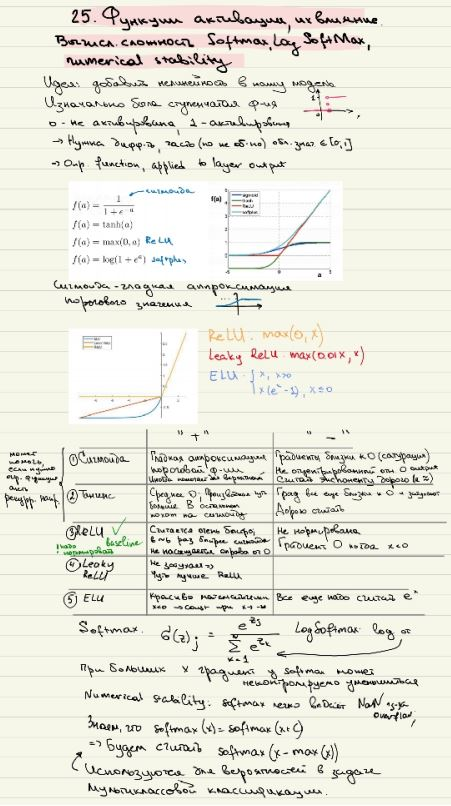
\includegraphics[width=350pt]{images/25.JPG}
\newpage

\section{Optimization methods in Deep Learning. Gradient descent, SGD, it upgrades: \\ Momentum, RMSProp, Adam.}
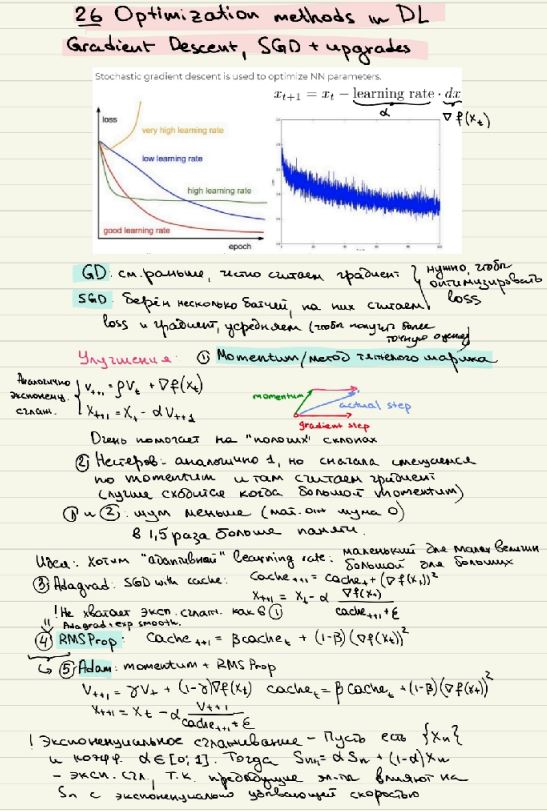
\includegraphics[width=400pt]{images/26.JPG}
\newpage

\section{Regularization in Deep Learning: Dropout, Batch \\ Normalization. Differences in training and evaluation stages.}\label{27}
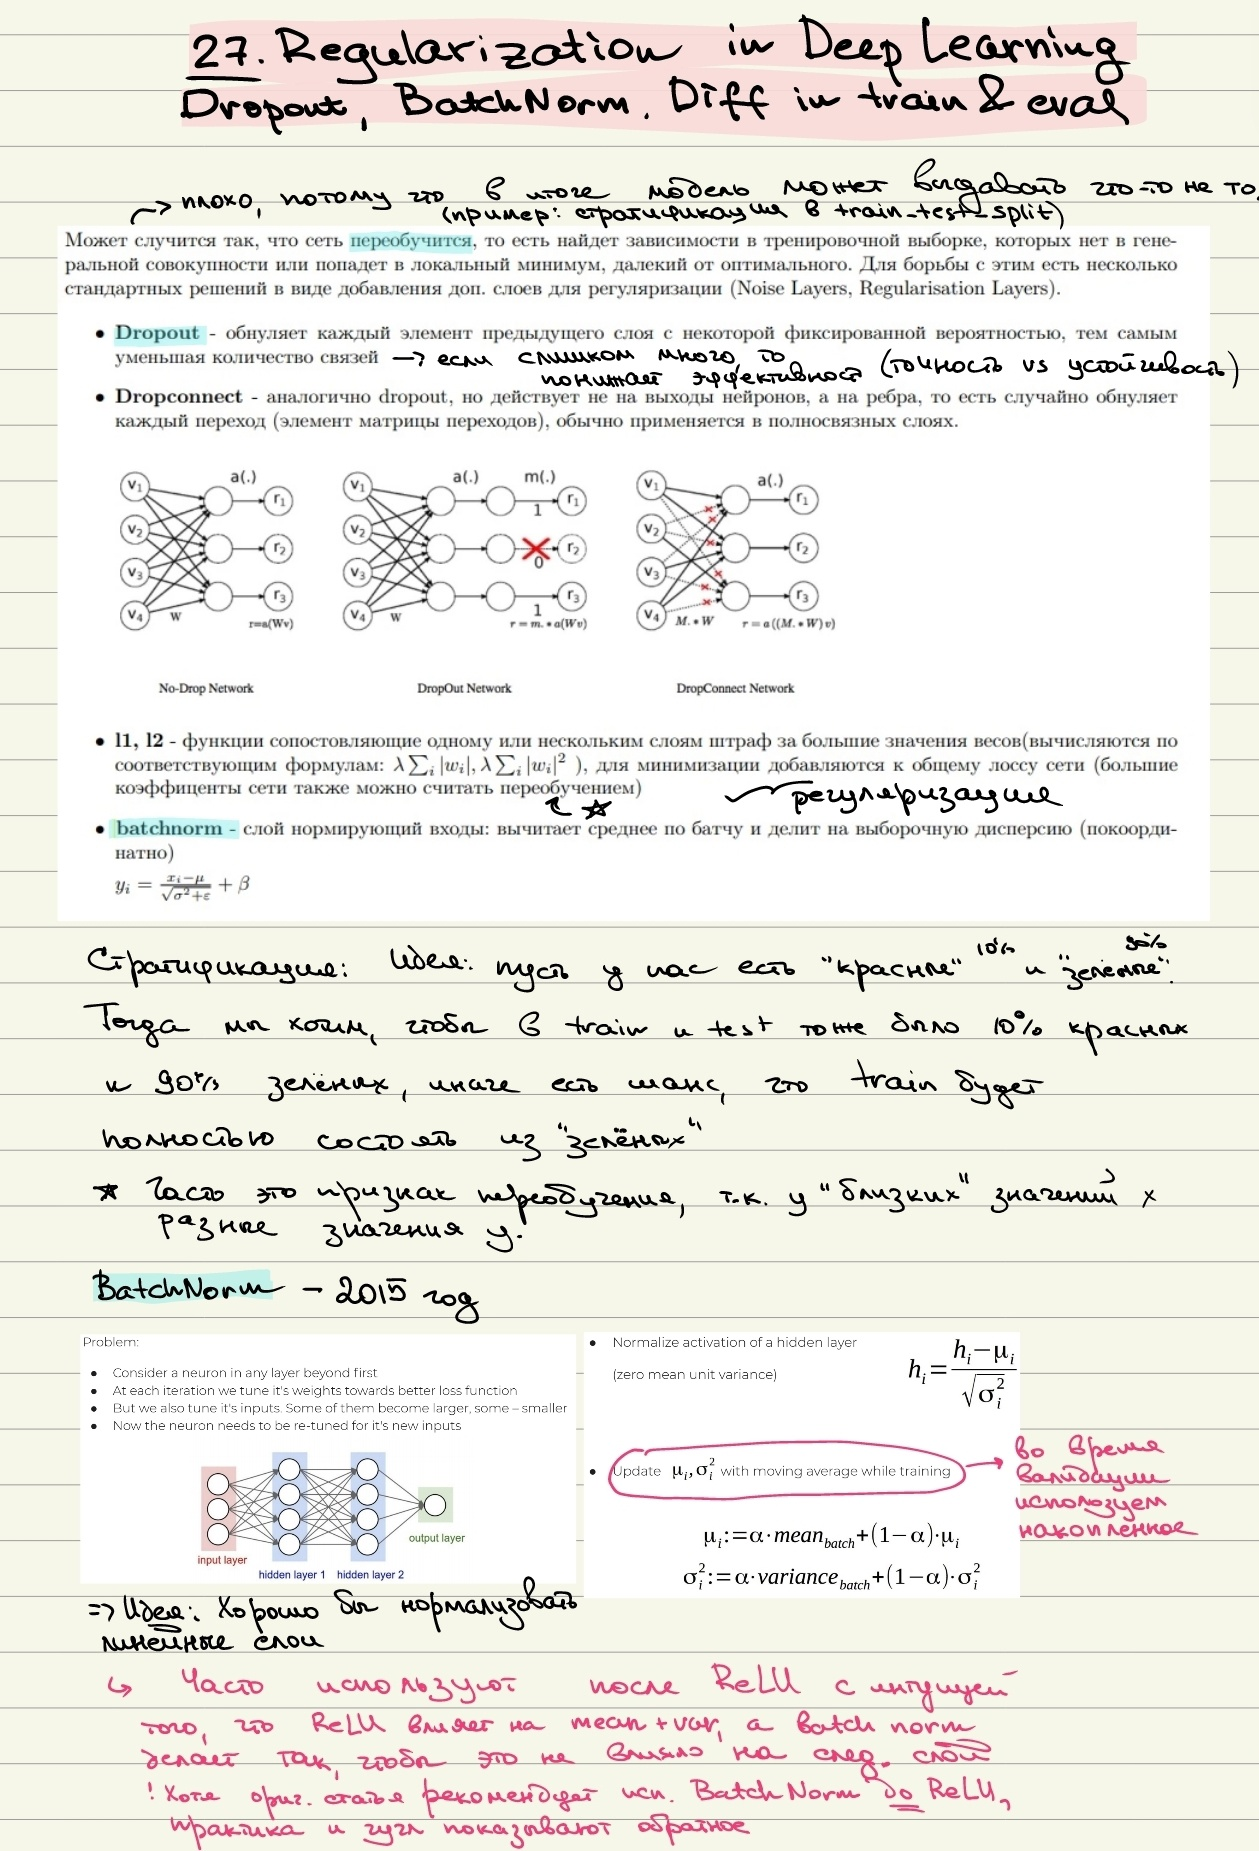
\includegraphics[width=400pt]{images/27_1.JPG}

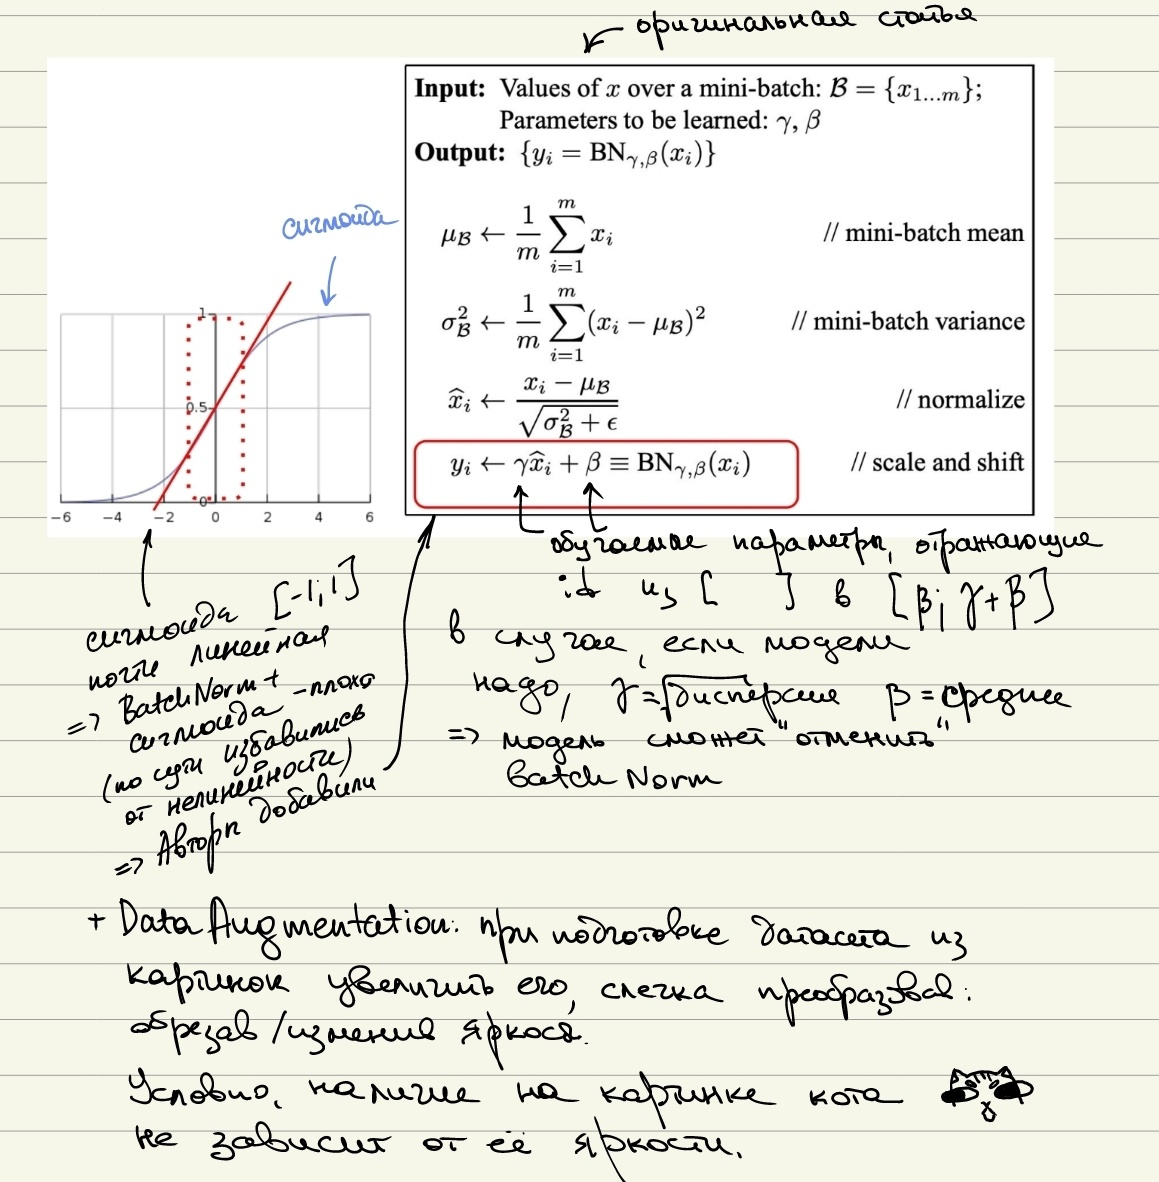
\includegraphics[width=400pt]{images/27_2.JPG}
\newpage

\section{Vanilla Recursive NN cell. Backpropagation through RNN. Vanishing gradient problem. Potential solutions.}
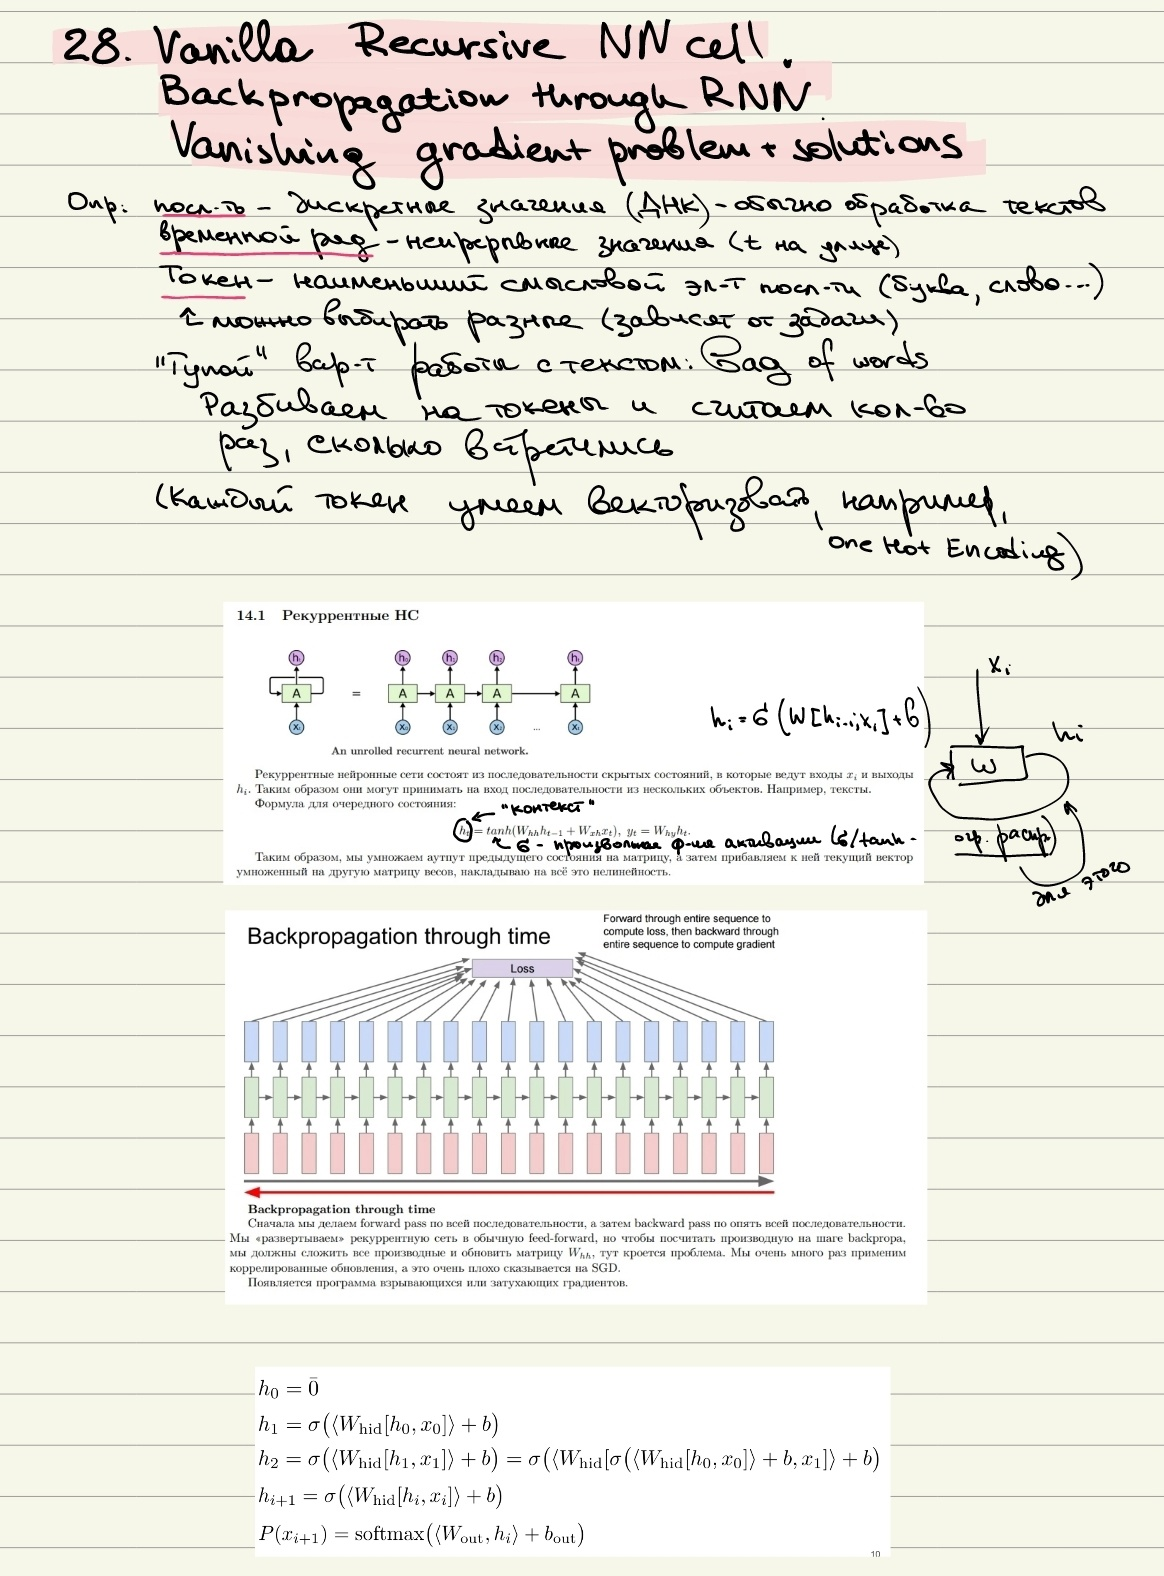
\includegraphics[width=400pt]{images/28_1.JPG}

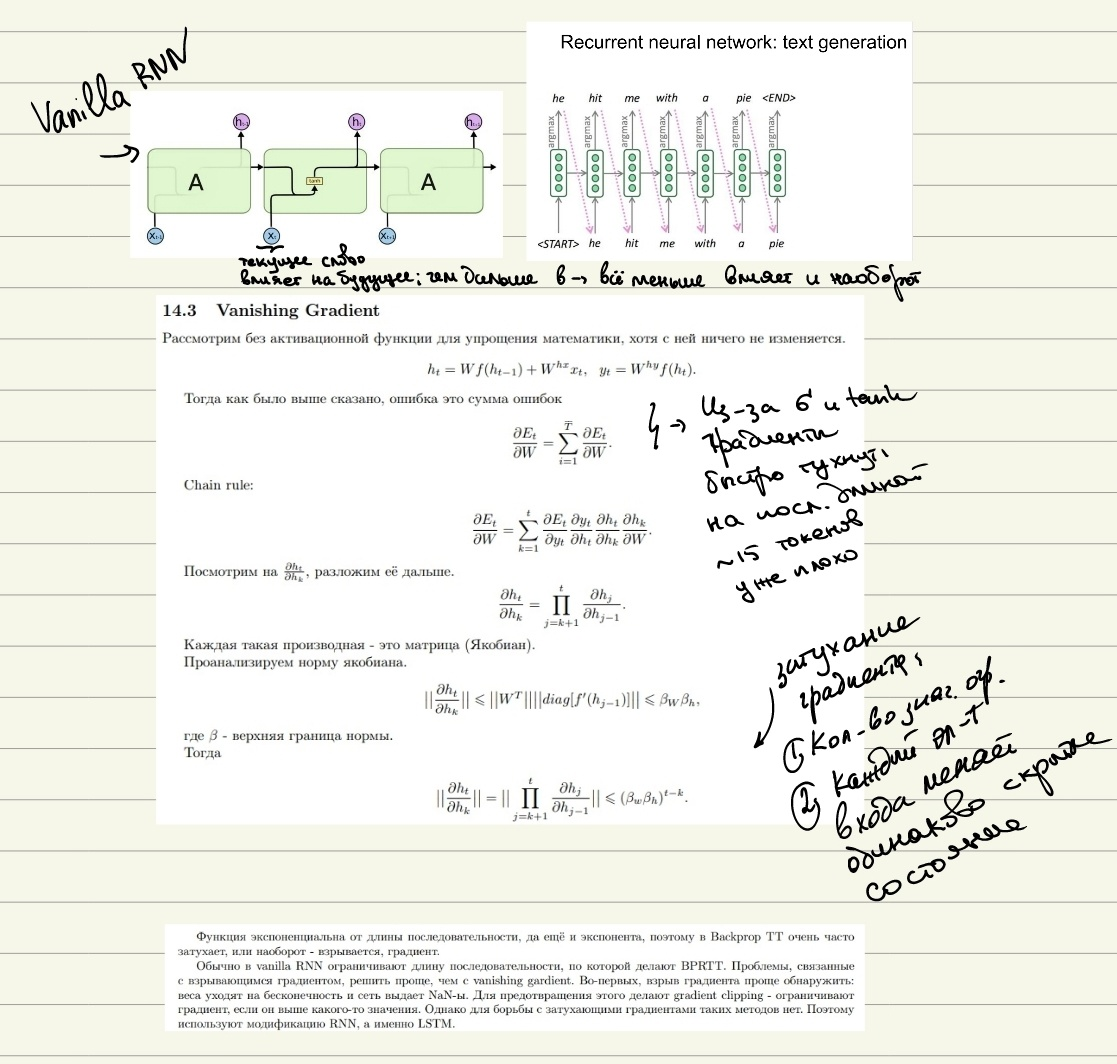
\includegraphics[width=400pt]{images/28_2.JPG}
\newpage

\section{LSTM/GRU, memory concept, gates ideas.}
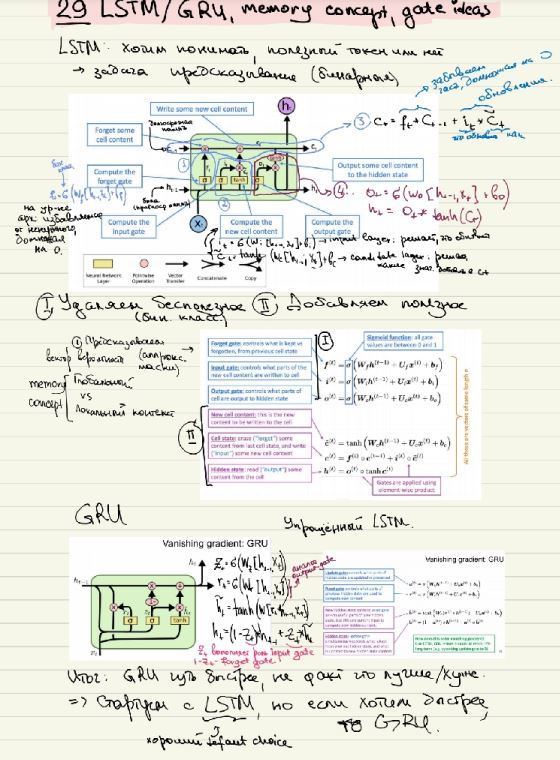
\includegraphics[width=450pt]{images/29.JPG}
\newpage

\section{Matrix convolution. Convolutional layer, backpropagation \\ through it. Hyperparameters of Convs. 1x1 convolutions, comparison to FC layers. Max/Average Pooling.}
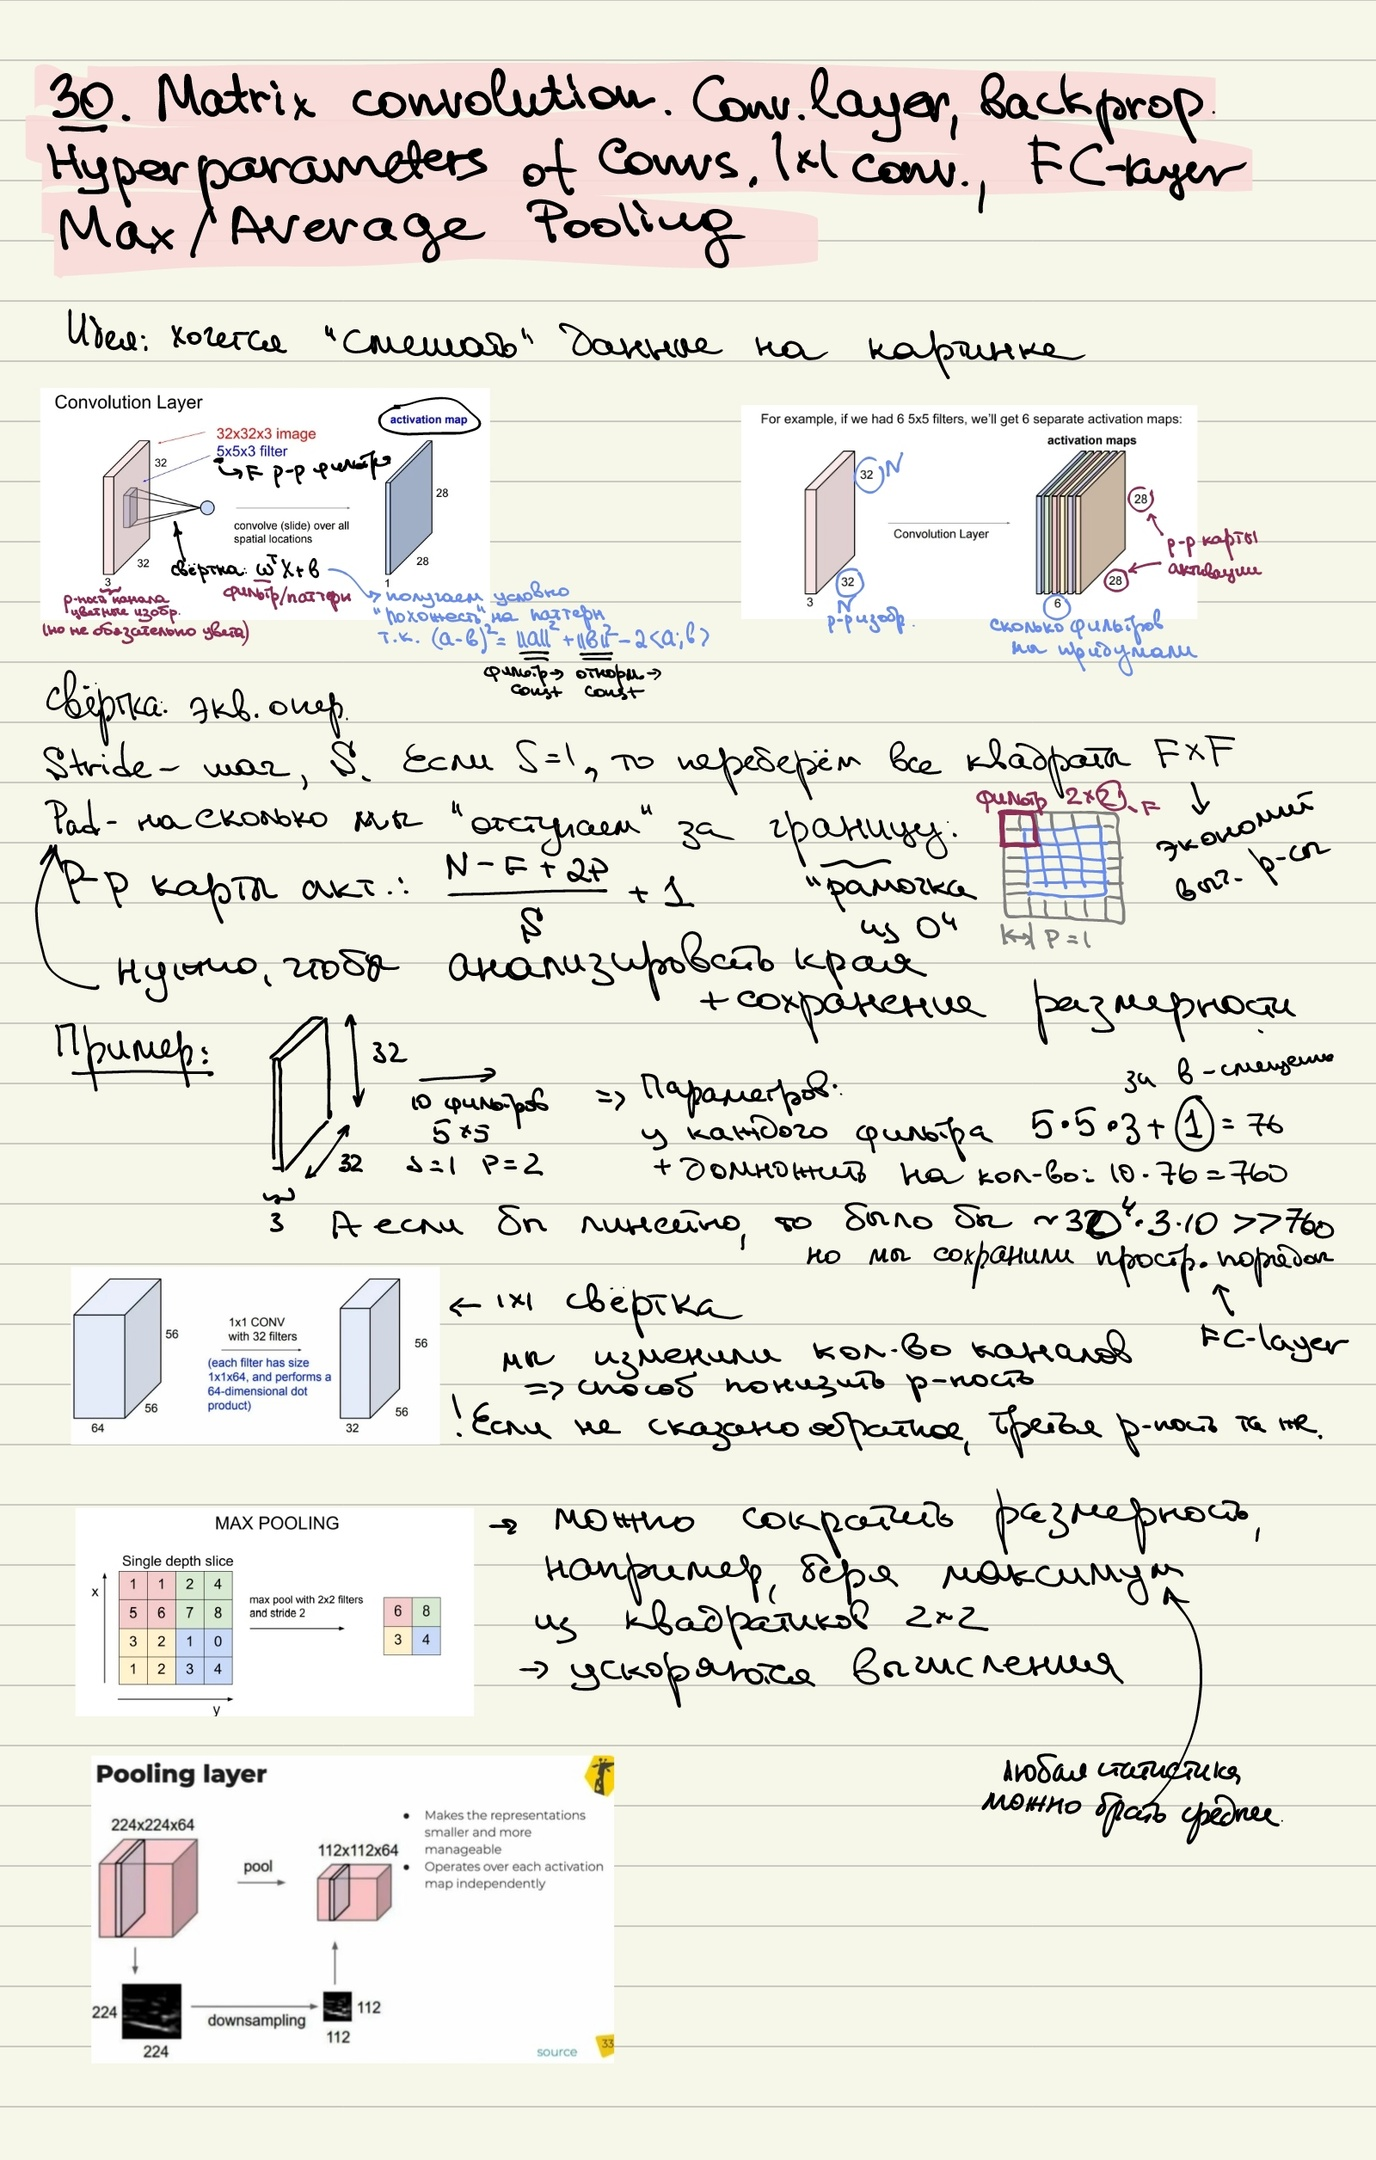
\includegraphics[width=400pt]{images/30.JPG}
\newpage

\section{Main ideas of AlexNet, VGG, Inception (GoogLeNet), ResNet architectures.}
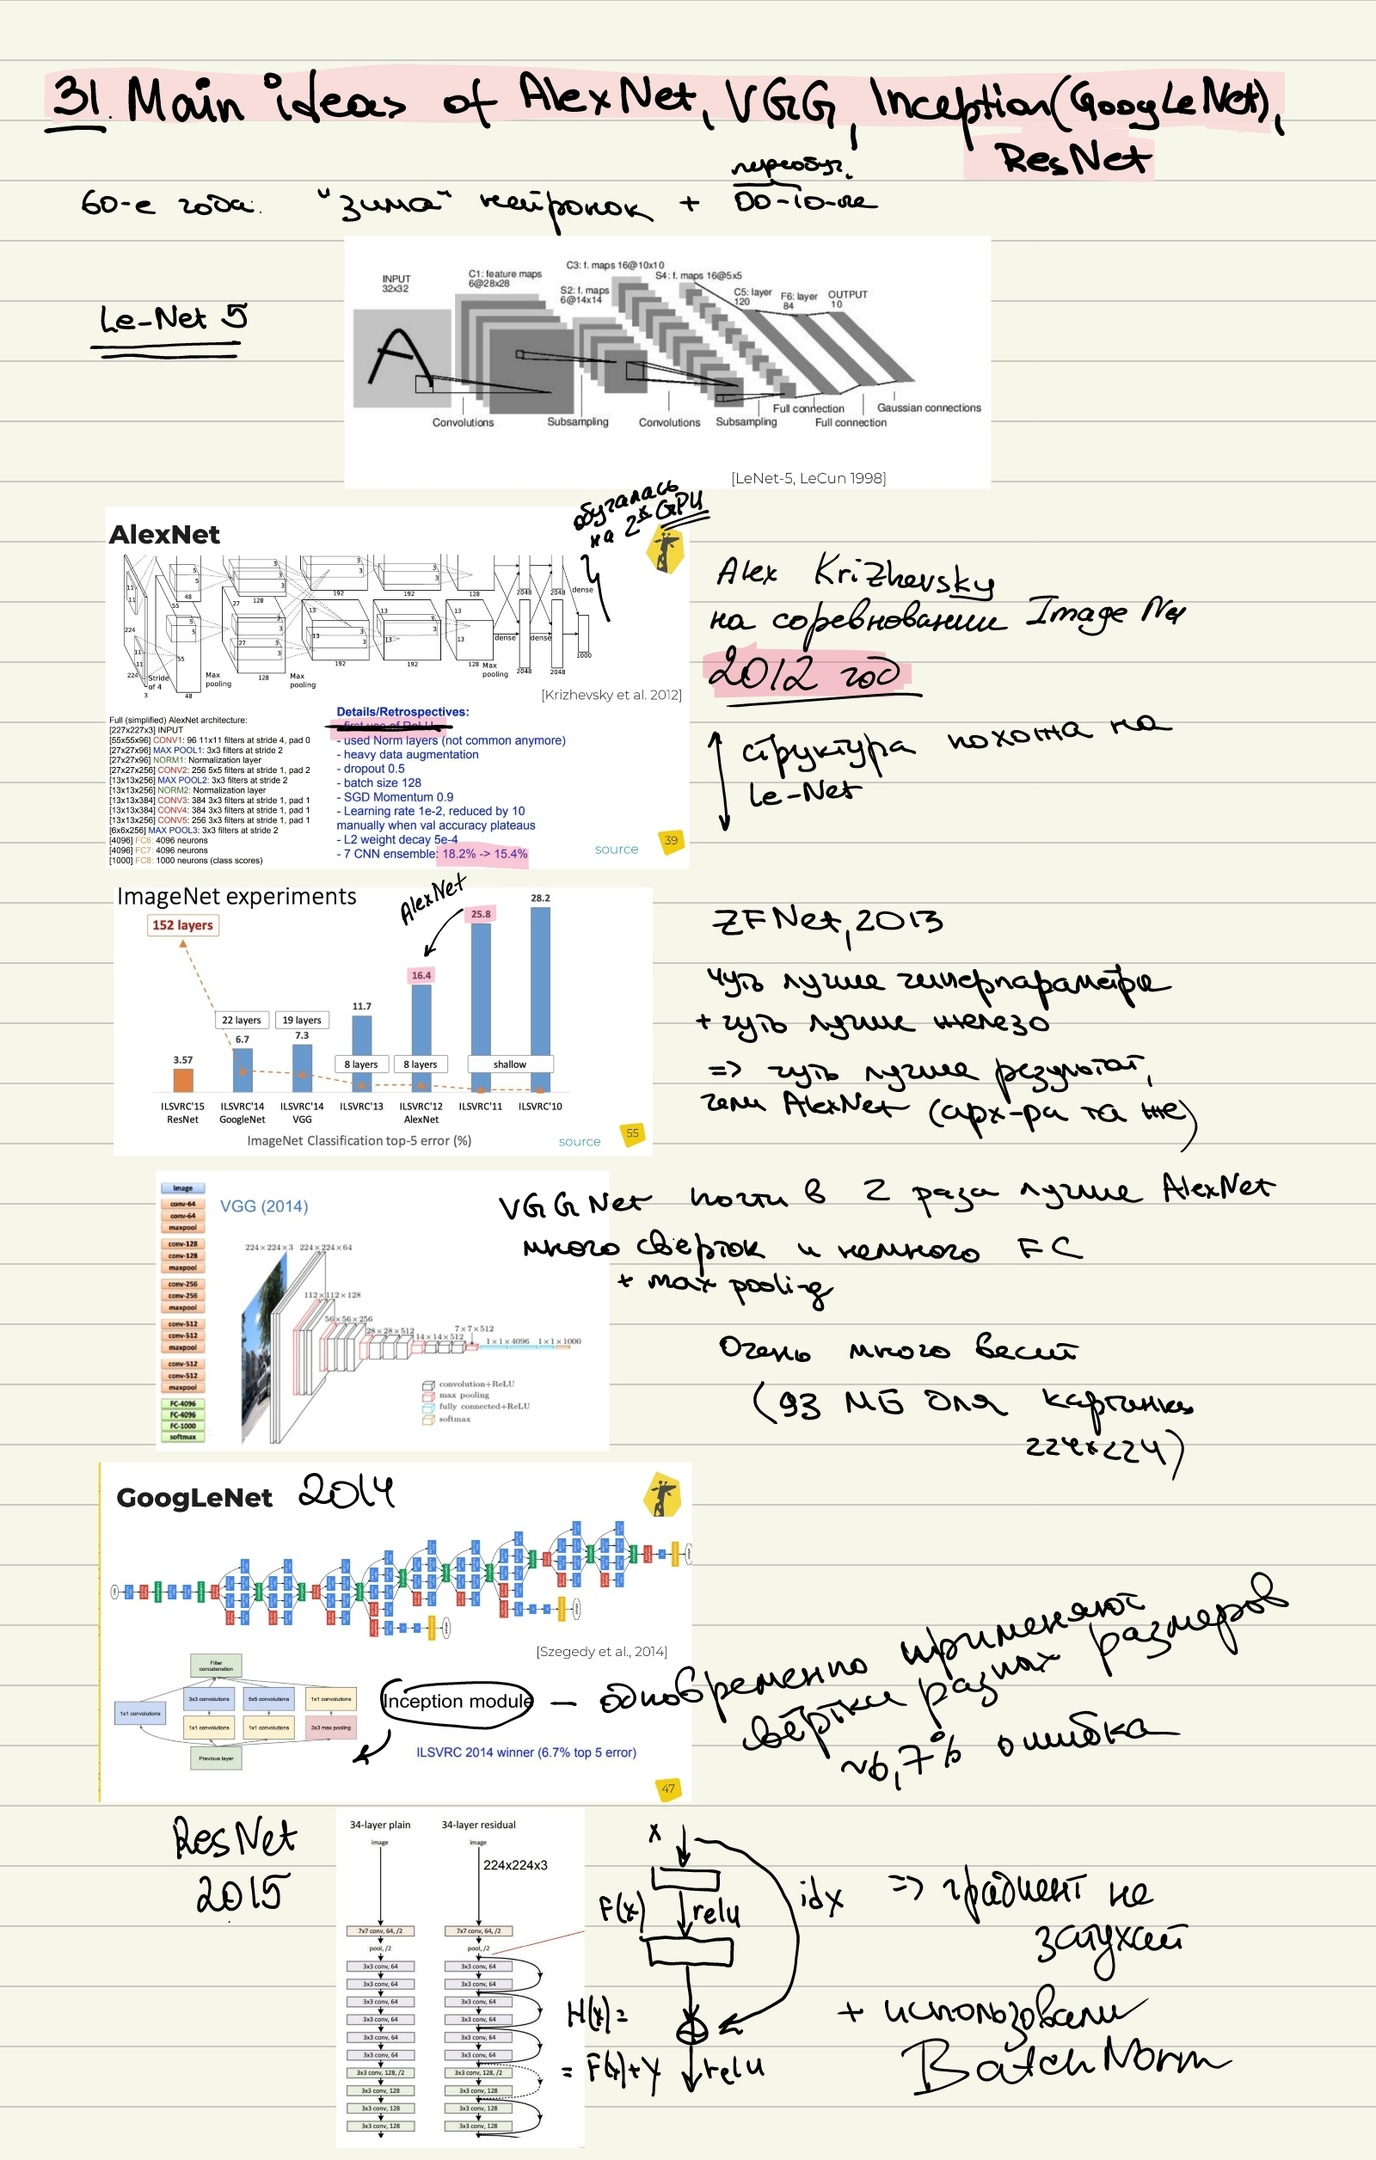
\includegraphics[width=400pt]{images/31.JPG}
\newpage

\section{Geometrical methods in ML. Clustering problem. IsoMap, LLE, DBSCAN, k-means, t-SNE}

\end{document}
